\documentclass[a4paper]{article}
\renewcommand{\baselinestretch}{1.5} 
\usepackage[toc,page]{appendix}
\usepackage[T1]{fontenc}
\usepackage[utf8]{inputenc}	
\usepackage[english]{babel}
\usepackage{titlesec}
\usepackage{color}
\usepackage{graphicx}
% \usepackage[fontsize=14]{scrextend}
\usepackage{fancyhdr}
\usepackage{listings} % for showing code snippets
\usepackage{caption} % for fancy titles
\usepackage{geometry}
\usepackage{varwidth}
\usepackage{chngpage}
% \definecolor{lBlue}{RGB}{3, 207, 252}
\definecolor{purple}{RGB}{240, 105, 255}
\usepackage[justification=centering]{caption} % to center multiline captions 
\captionsetup{format=plain, labelfont={color=purple,bf,it} } % for colored caption labels
\usepackage{array}
\usepackage{makecell}
\usepackage{float}
\usepackage{csquotes} % used for quote env
\usepackage{pdfpages}
\usepackage{svg}
\usepackage{amsmath} % for equations
\usepackage{nameref} %for ref of section name
\usepackage[noabbrev]{cleveref}
\usepackage[toc,page]{appendix}
\usepackage[style=ieee, backend=biber]{biblatex}

\bibliography{bibl.bib}
\addbibresource{bibl.bib}
\include{bibl.bib}

\graphicspath{{pictures/}}

\let\origthelstnumber\thelstnumber
\makeatletter
\newcommand*\Suppressnumber{%
  \lst@AddToHook{OnNewLine}{%
    \let\thelstnumber\relax%
     \advance\c@lstnumber-\@ne\relax%
    }%
}

\newcommand*\Reactivatenumber[1]{%
  \setcounter{lstnumber}{\numexpr#1-1\relax}
  \lst@AddToHook{OnNewLine}{%
   \let\thelstnumber\origthelstnumber%
   \refstepcounter{lstnumber}
  }%
}
\newcommand{\comment}[1]{}  % adds a new command \comment which does nothing. So everything defined in it will be ignored

\definecolor{sBlue}{RGB}{0,92,178}
\definecolor{ssBlue}{RGB}{30,136,229}
\definecolor{sssBlue}{RGB}{106,183,255}
\definecolor{gray75}{gray}{0.75}
\newcommand{\hsp}{\hspace{20pt}}
\titleformat{\section}[hang]{\Huge\bfseries}{\thesection\hsp{|}\hsp}{0pt}{\Huge\textcolor{sBlue}}
% \titlespacing{\section}{1cm}{*0}{*0}
\titleformat{\subsection}[hang]{\Large\bfseries}{\thesubsection\hsp}{0pt}{\Large\textcolor{ssBlue}}
\titleformat{\subsubsection}[hang]{\large\bfseries}{\thesubsubsection\hsp}{0pt}{\large\textcolor{sssBlue}}
\pagestyle{fancy}
\fancyhf{}
% \title{Gaming Systems}
\title{Orchestration on the Edge -\\ An Empirical Use Case of Kubernetes for Edge Computing}
\author{Jonas Burster - 20165136\\jburst16@student.aau.dk}

\date{xx.xx.2019}
\pagestyle{fancy}
\makeatletter
\let\runtitle\@title
\let\runauthor\@author
\makeatother
\lhead{\runtitle}
\rhead{Jonas Burster}



\begin{document}
% \includepdf[pages=-]{PDF/page_0.pdf}
% \maketitle

% \begin{figure}
% \vspace{-18cm}
%     \centering
%     \includegraphics[scale=0.4]{agillic-full-product-ball.png}
%     \label{fig:agillic-logo}
% \end{figure}
% \clearpage



\cfoot{\thepage}
\pagenumbering{Roman}

%\citetrackerfalse
\clearpage
% \tableofcontents
% \listoffigures
\clearpage

\pagenumbering{arabic}
% \section{Glossary - either before report or after report -breaks reading flow!}
\section{Introduction - Frame it as a video IoT problem. IoT is nice but video in IoT is hard to manage especially live data. How to cope with a lot of real time data examplified in the leading video surveilance company.}
\subsection{Motivation - More reference; Less technical --> building better scalability and flexbility, modular vs monolithic, cloud --> Don't be so technical, more highlevel and grandual go into real challenges}
\subsection{Problem Definition}
\section{Methodology - Could also be in Introduction (if more than 1 page)}
\section{Motivate why Cloud is important to milestones --> Enabling surveilance in the cloud. Collecting data from video cameras and building flexible scaling service architecture around that, that can be extended upgraded to add functionalty and maintainability. Service Mesh is relevant for Milestone.}
\section{History of Microservice Architecture - integrate SOA from paper - lose coupling!!! using descriptive messages rather de; microservice came from SOA; Network function virtualization and software defined network (only look at it)}
\section{State of the Art (Competitor analysis)}
\section{Literature Review/ What is a Service Mesh --> merge with history}

\section{Requirements from Milestone}
\subsection{Interviews (Head of Research and Cloud Orchestration Lead + With Professional from Istio Gathering in Cph)} 
\subsection{Functional Requirements ; Each Req should have source and reason}
\subsection{Non-Functional Requirements; source and reason}
\subsection{MoSCoW --> Give reason for prioritize certain feature (discuss what I can do and lower priority could be part for future.}
\section{Istio}
\subsection{Capabilities - Consider removing this. }
\subsection{Testing Istio Overhead in a Generic Setup}

\section{Implementation in Milestone}
\subsection{The current C2C? setup at Milestone}
\subsection{Platform Improvements from Istio}
\subsection{Chaos Testing}
\subsection{Benchmarking before vs after}
\section{Reflection/ Evaluation}
\section{Future Work}
\section{Conclusion}





% \section{Glossary}

- explain the major technologies and concepts\\
- Keep simple and short ( use same reference style for outside\\ literature)\\
- 

\subsection{Internet of Things}
The Internet of Things (IoT) describes 

\subsection{Fog Computing}
Fog computing describes the architectural style of carrying out computation, storage and communication (locally) at the edge of the network \citep{fogComputing:def}. It thus brings with it a whole new set of problems and challenges compared to the cloud. According to \citep{Introducing:kubeedge}, a senior software engineer in the field cloud messaging and IoT platforms at Red Hat, its three main advantages over the cloud are: "Low latency, availability and locality". 

\subsubsection{OSI Model}
Similarly to the Kubernetes and Istio documentation this report will use the 7-Layer OSI model \cite{IstioLayers61:online}


\subsection{CI/CD}
CI/CD is an automated approach to software development. CI stands for continuous integration and means continuously merging working code with the master branch, while testing for code quality via unit and integration tests \citep{shahin2017continuous}. CD stands for continuous development (sometimes also deployment) and means running 
\section{Introduction}
\begin{displayquote}
\textit{\textbf{\Huge{``}}
\large{Around 10\% of enterprise-generated data is created and processed outside a traditional centralized data center or cloud. By 2025, Gartner predicts this figure will reach 75\%.\cite{gartnerEdgeComputing:online}}
\textbf{\Huge{''}}}
\\[1pt]
\raggedleft{{\rm --- Gartner}}
\end{displayquote}
Data has never been as ubiquitous as it is today. Not only do our mobile phones constantly generate data but also the things we wear, use and own are now generating data. Not only the private sector is effected by this data revolution also the industry is embracing new technologies to gather data to automate processes. Some factories are even operated entirely self-sufficient without any human intervention. These factories are called "lights-out factories" and are becoming more and more popular\cite{wheresmyRobotLightsOut33:online}. In a world where data is everywhere the computing power to process this data has to be everywhere as well. Relying solemnly on centralized servers will eventually topple the system. The estimate by Gartner that 75\% of data will be generated and processed outside traditional data centers clearly shows decentralized architectures are here to stay.\\
In a curated report from the economist in 2015 the authors conclude that "cloud computing has the potential to disrupt entire industries, reshape businesses and markets and change the way we think about information"\cite{PuttogetEconomistCloud13:online}. Much of this success can be attributed to Kubernetes. It is a platform for container orchestration and was donated by Google to the open source community in 2014\cite{WhatisKubernetes87:online}. It enables the abstraction of hardware from deployments and provides much of the simplicity of Platform as a Service (Paas).\\
Edge computing is the term used for processing and storing data on the edge of the network. Fog computing is a subform of edge computing where the edge part is tightly integrated with the cloud to enhance both systems. This brings new possibilities and challenges to system designers.\\
In this thesis I will also construct an exemplary fog setup to remotely monitor and control lights to see the areas Kubernetes excels in but also it shortcomings. Finally, I will argue that Kubernetes should be the default platform for both cloud and edge computing to provide a homogeneous system for easy development, management and monitoring. Kubernetes is not fully optimized for this task yet, but the sooner it is the better for the entire industry.



% \comment{
In 2015, the Cloud Native Computing Foundry (CNCF) was founded under the 
umbrella organization of the Linux Foundation. 

https://blogs.gartner.com/thomas_bittman/2017/03/06/the-edge-will-eat-the-cloud/

Since edge devices can also produce terabytes of data, taking the analytics closer to the source of the data on the edge can be more cost-effective by analyzing data near the source and only sending small batches of condensed information back to the centralized systems.
}
\subsection{Motivation}
Edge computing, and especially fog computing, are emerging as a new paradigm on how to structure the computational resources of a system. It enables technology to operate very close to the user or thing and places no additional burden on the core network or servers. According to Dejan Bosanac, a senior software engineer at Red Hat in the field of cloud messaging and IoT platforms, these devices have three main advantages over the cloud due to their proximity to the devices and end users: 
\begin{displayquote}
{\textbf{``Low latency, availability and locality''}}\cite{IntroducingDejanBosanac:KubernetesIoTEdgeWorkingGroup}
\end{displayquote} 
Edge computing is set to have profound changes on mobile computing and Industrial IoT (IIoT) and has been described as "enabler for the Industrial Internet of Things"\cite{steiner2016fogenablerIIoT} in the academic literature.

However, there is no industry wide standard for structuring or deploying edge resources. No software has yet emerged and taken the industry by storm and became the de-facto standard. Kubernetes has done so in the cloud and I am going to argue Kubernetes will be the technology to transform the edge from an isolated into an active part in the data processing pipeline. Importantly, Kubernetes not only has the advantage of fog computing, i.e. cloud aware edge device or enabling offline edge clusters, but also includes central and standardized monitoring and networking. As most systems will be connected to the Internet one way or another in the future, fog computing stands to be the primary use case, but it is not required.

For edge computing security, hardware restrictions, isolation, fault tolerance and more are immensely important issues and Kubernetes already has the tools and features to solve many of these problems. Importantly, Kubernetes allows for remote controlling and monitoring of systems and works actively to ensure the desired state of the cluster.

\comment{


In this thesis I will thus explore how Kubernetes can facilitate fog computing and what challenges still have to be solved.
}
\subsection{Problem Area}\label{sec:problemArea}
\comment{
Why are IoT Gateways so hard to get right? Why is the edge so hard to get right?
 - Diversity
 - Security
 - Stability
}
% Main text
{
Mobile devices profoundly changed the way computers interact with each other. When these devices became a commodity in the 90s\footnote{Back then smartphones were called personal digital assistant (PDA).}, the way we manage computing power needed to change to accommodate intensive tasks on light weight computers. Researchers started to experiment with local, remote (cloud) and mixed execution also called adaptive cloud offload. The researchers found huge gains from adaptive cloud offloading with a high enough bandwidth and concluded "the convergence of mobile computing and cloud computing enables new multimedia applications that are both resource-intensive and interaction-intensive."\cite{noble1997agileIoTGatewayOdyssey}. As one of the researches later put it "while mobile elements will undoubtedly improve in absolute ability, they will always be at a relative disadvantage."\cite{satyanarayanan2015briefHistoryIoTGateway}\\
Today, we not only have smartphones, which have gotten quite powerful, but tiny IoT devices which are often build to last months on a single battery and have very, very limited processing power. New architectural patterns and communication technologies emerged to support these ultra low power and processing requirements. This lead to a fractured landscape where many manufacturers developed their own technology, mostly as closed source. There were some open source efforts but none taking over the entire industry. It was not felt necessary to have a centralized control plane, where updates could be scheduled and the system monitored. Applications did not have any isolation from the host operating system and often times security updates were not even deemed necessary, which left many IoT gateways and devices vulnerable to attacks leading to serious attacks like the Mirai botnet\cite{7971869MiraiAndOtherBotnetLinux}. Its important to note, that most attacks target Linux devices and not microcontrollers running on real time operating systems (RTOS).\\
In 2009, the National Science Foundation rejected a paper because \textit{``Many panelists do not agree with the premise of the proposal in which distant cloud computing incurs too high latency to be acceptable by mobile applications. They question the validity of such assumption as the proposal provides no real data to justify it[...]''}\cite{satyanarayanan2015briefHistoryIoTGateway}. Much has changed since then. The smartphone revolution greatly increased the data produced by mobile devices and the need for speed, security and privacy. Researches did not foresee the explosion in IoT and the onset of a new wave of data producers bundled under the term Indutrial IoT (IIoT). It includes hundreds and thousands of IoT devices working together in factories, logistic warehouses, connected vehicles (CV), smart grid etc. In 2012 a widely cited paper "Fog Computing and Its Role in the Internet of Things"\cite{fogComputing:def} was published, establishing the need for IoT gateways connected to the cloud. It concluded that the amount and high frequency of produced data is too much for the cloud and pre-processing on the edge is needed for both latency and efficiency.\\
However, establishing the need for edge computing is not the same as solving it. Since then many papers have been published with titles such as "The Internet of Things Has a Gateway Problem"\cite{zachariah2015internetOfThingsHasGatewayProblem}. At the same time, researchers used custom IoT gateway solutions and achieved impressive results. In one experiment, they achieved over 80\% performance increase in certain scenarios rightly titling their paper "From Cloud Computing to Fog Computing: Unleash the Power of Edge and End Devices"\cite{hong2017fromCloudtoIoTGatewayUnleashingTHePower}.\\
}

\subsubsection{Expected Outcome}
This thesis will implement a fog system with Kubernetes at its core. It will explain how Kubernetes can aid in many challenges facing the edge and give insights into Kubernetes resources important for the edge, including containers, and the best practices. Such a system could become the industry norm influencing millions of deployments in many diverse industries. It would improve communication and observability and finally put a halt to most malicious attacks by reducing the attack surface to a bare minimum.\\

\subsubsection{Research Question}
In essence, the research question for this thesis is:
\begin{displayquote}\begin{center}
{\textit{\textbf{How can Kubernetes facilitate edge computing, what challenges does it solve and where are its shortcomings?}}}
\end{center}\end{displayquote}

\subsubsection{Delimitation} \label{sec:delimitation}
\comment{
Exclude non Kubernetes related technologies.\\
Exclude mobile devices.\\ All a lot of technologies are still relevant but not discussed. In future work mention it
Exclude hardware.\\
Exclude Sort of 5g and advances in mobile technologies.\\ Rich field
Exlude infrastructure edge.\\
Exclude RTOS.\\
}








\comment{


Edge computing started as a way to give mobile devices more power.
Technopedia defines a mobile device as a "handheld tablet or other device that is made for portability, and is therefore both compact and lightweight"\cite{WhatisaM95TechnopediaMobileDevice:online}, it includes laptops, smartphones, tables etc.  As Mahadev Satyanarayanan put it "while mobile elements will undoubtedly improve in absolute ability, they will always be at a relative disadvantage."\cite{satyanarayanan2015briefHistoryIoTGateway} Back then, researchers experimented with local, remote (cloud) and mixed execution also called adaptive
cloud offload. Assessing the three variants for voice recognition, video playback and web browsing locally, the researchers found huge gains from adaptive cloud offloading with a high enough bandwidth and concluded "the convergence of mobile computing and cloud computing enables new multimedia applications that are both resource-intensive and interaction-intensive."\cite{noble1997agileIoTGatewayOdyssey}. This lead to an explosion in cloud development. The Internet started out with a decentralized servers around the world. But over the years technologies were invented for orchestration across these distant servers, but also isolation for the local deployments. Probably the two main technological standards evolving where containers with containerd and orchestration with Kubernetes. \\
Traditionally, mobile devices connected to a gateway, which was mainly a router operating at L3\footnote{L3 stands for Layer 3, the networking layer in the OSI model.} to route packets and translate between different types of network protocols. \cite{lee2017futureOfIoT}. However, according to Dejan Bosanac, a senior software engineer at Red Hat in the field of cloud messaging and IoT platforms, due to their proximity to the sensors and the end user, these devices have three main advantages over the cloud: 
\begin{displayquote}
{\textbf{``Low latency, availability and locality''}}\cite{IntroducingDejanBosanac:KubernetesIoTEdgeWorkingGroup} - Dejan Bosanac.
\end{displayquote}
Because of these advantage researchers construct hybrid systems, in which devices operating on the edge of the network play an active role in the data processing pipeline. This architectural style of carrying out substantial amount of computation and storage at the edge is called "edge computing" \cite{fogComputing:def}. \Cref{fig:iotDeviceSetup} shows where the gateway is positioned in the current communication setup. 
 \begin{figure}[!h]
     \centering
     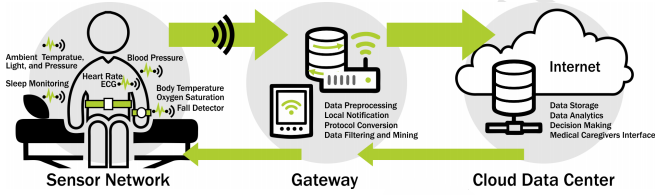
\includegraphics[scale=2]{figures/iotSetup.png}
     \caption{The position of the gateway in the current Internet infrastructure\cite{iotGatewaySlavesGraph}.}
     \label{fig:iotDeviceSetup}
 \end{figure}\\
But not everyone in the academic world was convinced that edge computing was indeed the way forward. 
However, establishing the need for edge computing is not the same as solving all problems though, and since then many papers have been published with titles such as "The Internet of Things Has a Gateway Problem"\cite{zachariah2015internetOfThingsHasGatewayProblem}. At the same time, researchers used custom IoT gateway solutions in their research and achieved impressive results. In one experiment, they achieved over 80\% performance increase in certain scenarios rightly titling their paper "From Cloud Computing to Fog Computing: Unleash the Power of Edge and End Devices"\cite{hong2017fromCloudtoIoTGatewayUnleashingTHePower}. Adding further to the problem of standardization is that IoT, especially IIoT, and mobile device have very different requirements.\\
This is the current place of the industry. There is a common agreement that fog computing is essential in the future, but no standard and open solution was developed yet. There is considerable effort in the academic world and in the industry to establish such a standard, one such initiatives is the Kubernetes IoT Edge working group under the Cloud Native Computing Foundry (CNCF). 




The space between the cloud and IoT and mobile devices, can be confusing at times. Knowing the history of IoT and the cloud is vital to understand the current developments. This, the methodology and the delimitation of this thesis will be discussed in the reminder of this section.\\




The terms used in the academic world and the industry are often different and many concepts partially overlap and complement each other making it hard to clearly categorize solutions. This is mainly due to ever evolving hard- and software, changing the possibilities of the devices and the entire landscape. It is thus imperative to clearly outline the key terms and design philosophies used of this thesis as well as presenting already existing solutions and how they compare to each other. These aspects are part of \cref{sec:eSOTA}, \nameref{sec:eSOTA}.\\
\Cref{sec:analysis}, \nameref{sec:analysis}, will lay the foundation to the actual implementation. We will motivate our design choices with academic and industry literature as well as with interviews from industry leaders. The focus of this thesis will be on the software and the requirements of the software to define and use the edge. Ultimately, it does not matter whether increases in performance and security come from better hardware or software, as long as the requirements are met. Consequently, the requirements will be ordered via the MoSCoW method. I will analyze the existing protocols, mainly for the application layer, and the data serialization method. Kubernetes is at the heart of this thesis implementation and extra sections will discuss what tricks Kubernetes already offers to control an edge cluster from the cloud and what might be missing. Additionally, I will look at extensions Kubernetes offers and how they could be useful in an IoT environemnt.\\


}

\comment{
The main focus is going to be on the software driving fog computing with an emphasize on IoT device and less mobile devices. 
We use a three tier layered network topology shown in \cref{fig:networkTopology3Layer}.
\begin{figure}[h!]
    \centering
    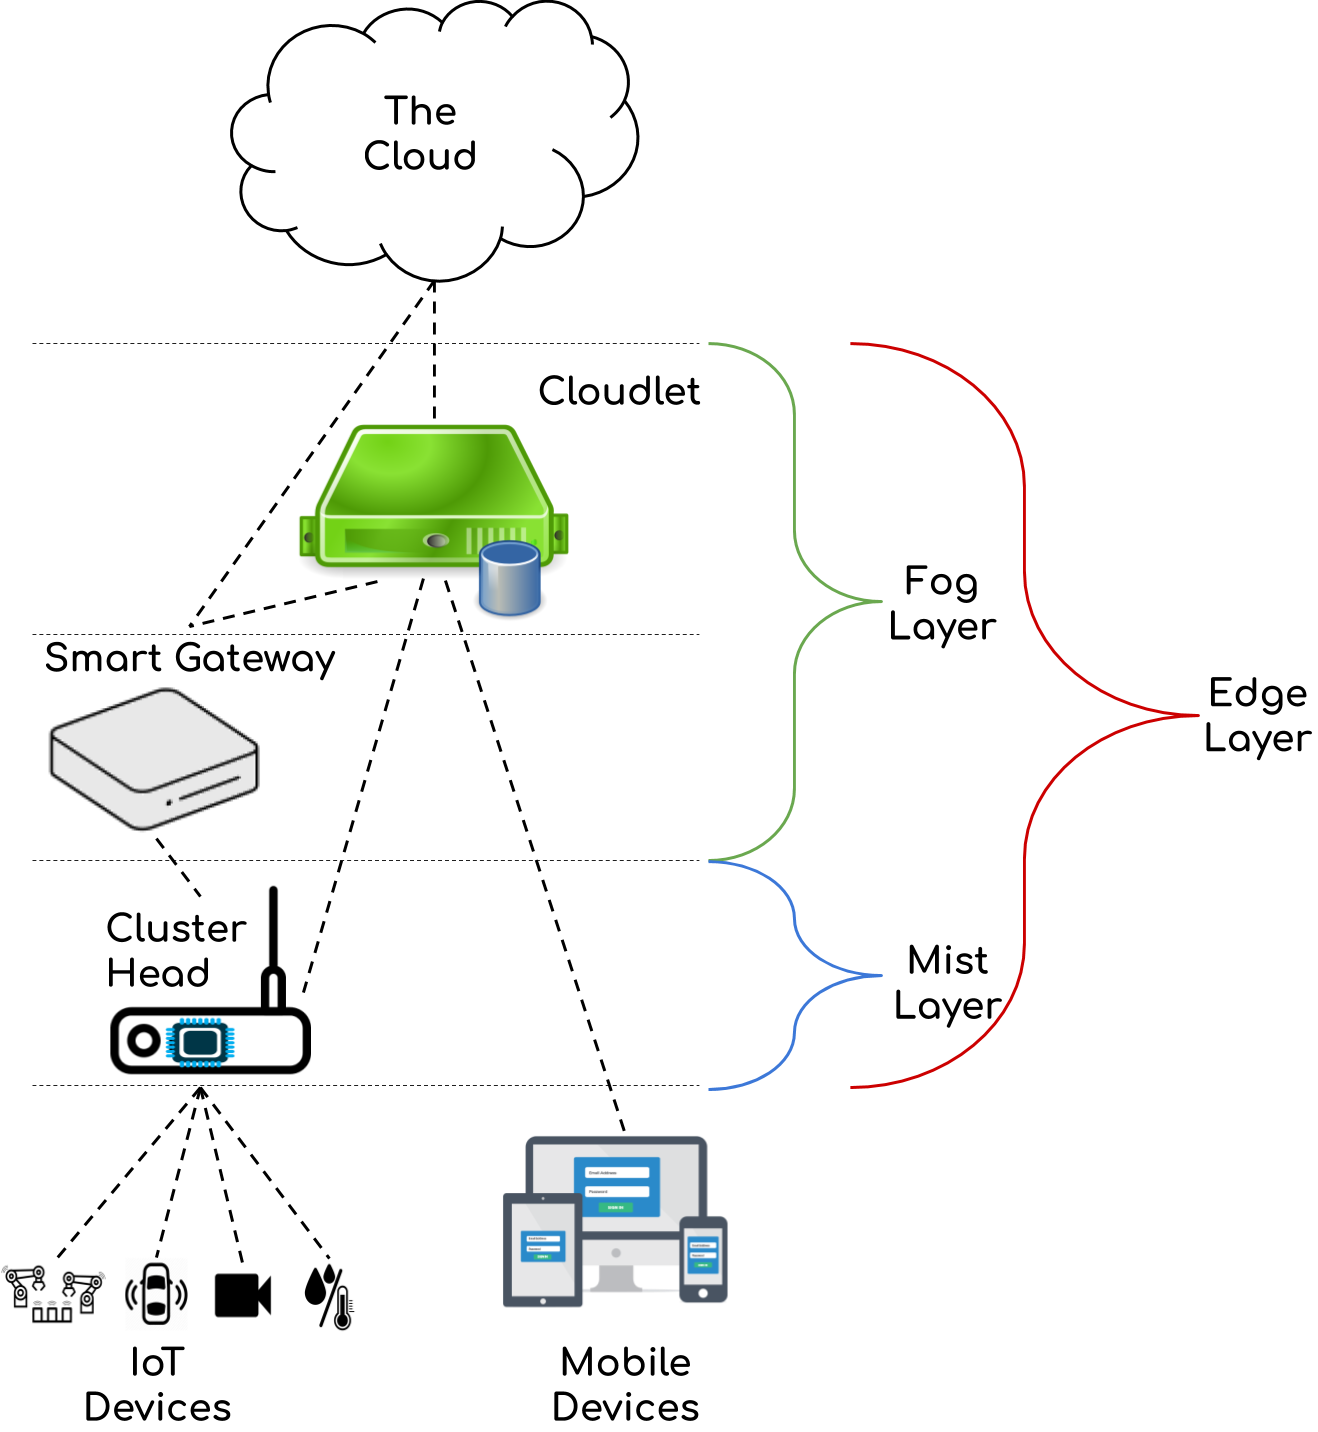
\includegraphics[scale=0.15]{figures/network-topology-3-layer.png}
    \caption{Three tier layer network topology, similar to \cite{nsa2017theNextWaveIoTDefinitions}}
    \label{fig:networkTopology3Layer}
\end{figure}
% Describe figure:
The cloud layer is made up of the 

% More detail
The cloud is the one layer where the authors think the technology stack is set. We expect Linux and Kubernetes, the de-facto standard for cloud orchestration, to be here to stay for the foreseeable future. This implies the same for x86\_64 and ARM, the only CPU architectures being supported by Linux. The Internets communication will remain in IPv4 and increasingly IPv6 for the Internet layer and TCP and UDP for the transport layer.\\ 
Quite the contrary is true for the bottom layer, IoT devices and mobile devices, although for the latter to a lesser extend. Communication in the IoT space is very diverse. Some protocols like 802.11 and Mobile

We expect IoT devices to have different software and different 
This can, but must not, include a control plane
The aim is to find the most promesing solution and 




Promesing solution with deep integration into K8s.


In essence, fog is the standard, and edge is the concept. Fog enables repeatable structure in the edge computing concept, so enterprises can push compute out of centralized systems or clouds for better and more scalable performance.
https://www.cisco.com/c/en/us/solutions/enterprise-networks/edge-computing.html


As it's name implies its aim is to develop an edge solution with Kubernetes support.

The need for smart IoT Gateways or fog computing is well established. They make it possible to 

Their design however is not. 
While the problems at the IoT edge — connectivity, manageability, scalability, reliability, security — are being solved as point solutions by enterprises and ecosystem players, there is a need for a foundational industry-wide standard for managing distributed IoT workloads.





IoT has seen a rapid growth over the last few years. According to IoT Analytics the total number of IoT devices is set to surpass the total number of other connected devices around 2021 \cite{StateofIoT:online}. Further, most IoT devices will be used in WPAN \footnote{Wireless Private Area Networks includes technologies like Zigbee,Z-wave and Bluteooth} and WLAN\footnote{Wireless Local Area Networks includes mainly Wi-Fi}. 
% In contrast to 5G, these technologies don't connect to an access point from an Internet provider but rather require another user operated device to connect to the Internet, a so called "gateway"


But fog computing does not come without its drawbacks. Depending on the protocol edge devices need to be close to their peers and slaves and physically accessible for maintenance. Which also poses a major security risk as they could be accessed by malicious intruders. The software maintenance is another critical aspects. Often IoT and edge devices are not update and patched with critical consequences. The "2016 Dyn cyberattack" used IoT devices like residential gateways, smart fridges, baby phones ect. to bring down the DNS-Servers operated by Dyn making large part of the Internet unaccessible for hours\cite{dynAttack}. The authors also stress that "large number of IoT devices are accessible over public Internet" and that "security (if considered at all) is often an afterthought in the architecture of many wide spread IoT devices"\cite{dynAttack}.\\
The question is then, how can manage and secure those devices. In this thesis, I will solely be concerned with the software aspect, which can mitigate some effects of exposing physical hardware to more accessible places.\\
Many challenges facing edge devices today have already been solved, although in a slight different context: The cloud\cite{IntroducingDejanBosanac:KubernetesIoTEdgeWorkingGroup}. In the cloud 




% Note: Maybe make a graph cloud setup, user connecting to nodes, VS fog computing, sensors and users connecting to gateways and gateway to cloud.  https://www.einfochips.com/blog/iot-gateways-drivers-for-fog-computing/

Kubernetes IoT Edge Working Group is a collaboration between Eclipse IoT Working Group and its 40-member companies, 35 open source projects, and Kubernetes ecosystem. It will define terminology, identify gaps in deployment and management, and educate the market on common use cases.
https://www.dailyhostnews.com/eclipse-foundation-and-cncf-working-together-to-bring-kubernetes-to-iot-edge
}
% \subsubsection{A Brief History}
\comment{
Why are IoT gateways important?
How did it come to be?
How did it start?
Why is it now, that many companies have interest?
}
Mobile devices profoundly changed the way computers interact with each other. Technopedia defines a mobile device as a "handheld tablet or other device that is made for portability, and is therefore both compact and lightweight"\cite{WhatisaM95TechnopediaMobileDevice:online}, it includes laptops, smartphones, tables etc. When these devices became a commodity in the 90s\footnote{Back then smartphones were called personal digital assistant (PDA).}, the way we manage computing power needed to change to accommodate intensive tasks on light weight computers. As Mahadev Satyanarayanan put it "while mobile elements will undoubtedly improve in absolute ability, they will always be at a relative disadvantage."\cite{satyanarayanan2015briefHistoryIoTGateway} Back then, researchers experimented with local, remote (cloud) and mixed execution also called adaptive
cloud offload. Assessing the three variants for voice recognition, video playback and web browsing locally, the researchers found huge gains from adaptive cloud offloading with a high enough bandwidth and concluded "the convergence of mobile computing and cloud computing enables new multimedia applications that are both resource-intensive and interaction-intensive."\cite{noble1997agileIoTGatewayOdyssey}. This lead to an explosion in cloud development. The Internet started out with a decentralized servers around the world. But over the years technologies were invented for orchestration across these distant servers, but also isolation for the local deployments. Probably the two main technological standards evolving where containers with containerd and orchestration with Kubernetes. \\
Traditionally, mobile devices connected to a gateway, which was mainly a router operating at L3\footnote{L3 stands for Layer 3, the networking layer in the OSI model.} to route packets and translate between different types of network protocols. \cite{lee2017futureOfIoT}. However, according to Dejan Bosanac, a senior software engineer at Red Hat in the field of cloud messaging and IoT platforms, due to their proximity to the sensors and the end user, these devices have three main advantages over the cloud: 
\begin{displayquote}
{\textbf{``Low latency, availability and locality''}}\cite{IntroducingDejanBosanac:KubernetesIoTEdgeWorkingGroup} - Dejan Bosanac.
\end{displayquote}
Because of these advantage researchers construct hybrid systems, in which devices operating on the edge of the network play an active role in the data processing pipeline. This architectural style of carrying out substantial amount of computation and storage at the edge is called "edge computing" \cite{fogComputing:def}. \Cref{fig:iotDeviceSetup} shows where the gateway is positioned in the current communication setup. 
 \begin{figure}[!h]
     \centering
     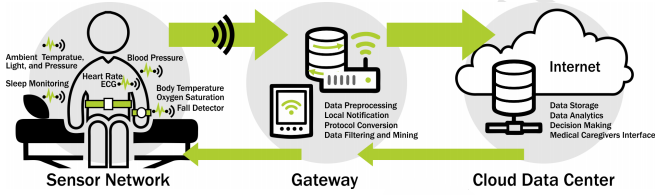
\includegraphics[scale=1.8]{figures/iotSetup.png}
     \caption{The position of the gateway in the current Internet infrastructure\cite{iotGatewaySlavesGraph}.}
     \label{fig:iotDeviceSetup}
 \end{figure}\\
But not everyone in the academic world was convinced that edge computing was indeed the way forward. In 2009, the National Science Foundation rejected a paper because \textit{``Many panelists do not agree with the premise of the proposal in which distant cloud computing incurs too high latency to be acceptable by mobile applications. They question the validity of such assumption as the proposal provides no real data to justify it[...]''}\cite{satyanarayanan2015briefHistoryIoTGateway}. Much has changed since then. The smartphone revolution (do I need to cite this? Is it a term I can actually use?) greatly increased the data produced by mobile devices and the need for speed and privacy. Researches did not foresee the explosion in IoT and the onset of a new wave data producers bundled under the term Indutrial IoT (IIoT). It includes hundreds and thousands of IoT devices working together, for example in factories, logistic warehouses, connected vehicles (CV), smart grid etc. In 2012 a widely cited paper "Fog Computing and Its Role in the Internet of Things"\cite{fogComputing:def} was published, establishing the need for IoT gateways connected to the cloud. The amount and high frequency of produced data is just too much to only handle in the cloud. Pre-processing on the edge is needed for both latency and efficiency.\\
However, establishing the need for edge computing is not the same as solving all problems though, and since then many papers have been published with titles such as "The Internet of Things Has a Gateway Problem"\cite{zachariah2015internetOfThingsHasGatewayProblem}. At the same time, researchers used custom IoT gateway solutions in their research and achieved impressive results. In one experiment, they achieved over 80\% performance increase in certain scenarios rightly titling their paper "From Cloud Computing to Fog Computing: Unleash the Power of Edge and End Devices"\cite{hong2017fromCloudtoIoTGatewayUnleashingTHePower}. Adding further to the problem of standardization is that IoT, especially IIoT, and mobile device have very different requirements.\\
This is the current place of the industry. There is a common agreement that fog computing is essential in the future, but no standard and open solution was developed yet. There is considerable effort in the academic world and in the industry to establish such a standard, one such initiatives is the Kubernetes IoT Edge working group under the Cloud Native Computing Foundry (CNCF). 


% \Cref{sec:problemArea}, \nameref{sec:problemArea}, will explain what challenges system designers face on the edge and why developing a standard is so hard.



























\subsection{Methodology}
The methodology describes the theoretical background for the methods applied in this thesis and ensures consistency across related work in the field.
The section Extended State of the Art is meant to provide the reader with an objective and complete overview of the research area. Following, in the Analysis section use cases are used to gather requirements. These are then prioritized according to the importance and feasibility for the desired system. Finally, in the Implementation, the system based on these requirements is implemented following a software development method and the priorities of the requirements.\\[5mm]
\textbf{\leftskip25mm\textit{Existing Solutions}}\\
The existing solutions section gives an objective presentations of already existing solutions in the field and sheds a light on how widely adopted systems or new once solve particular problems. It is not about the product but rather what the product tries to achieve and how.\\[5mm]
\textbf{\leftskip25mm\textit{Use Cases}}\\
Use cases are a way to find requirements\cite{UseCase94Fowler:online}. They can appear in the form of UML diagrams or written text. In this thesis only the written text version is used as the UML diagrams "[...]are of little value" and "the key value of use cases lies in the text" according to Martin Fowler\cite{UseCase94Fowler:online}. As the developed system is only a prototype I will use the "casual template for low-ceremony projects" from the book "Writing Effective Use Cases" from Alistair Cockburn\cite{cockburn2000writingUseCases}.\\[5mm]
\textbf{\leftskip25mm\textit{Functional Requirements}}\\
Functional Requirements state what services a system should provide, how it reacts to particular inputs, and how it should behave under particular circumstances\cite{sommerville2011software}. They are derived from the use cases and the state of the art and are the foundation for the implementation.\\[5mm]
\textbf{\leftskip25mm\textit{MoSCoW}}\\
The MoSCoW method is a way to structure the requirements according to the needs of the stakeholders involved\cite{sommerville2011software}. It is an acronym for "Must, Should, Could, Would". It helps to plan time and resources in a project so that the requirements with a higher ranking are finished first.\\[5mm]
\textbf{\leftskip25mm\textit{Agile Software Development Method}}\\
The software development method is a way to structure the development of software. An agile method emphasize development cycles to increase the transparency and flexibility during the software development. It decreases the risk of failure by constantly reevaluating the product. The agile manifest developed by industry experts\cite{beck2001manifestoAgile} has four main values: Individuals and Interactions over processes and tools; Working Software over comprehensive documentation; Customer Collaboration over contract negotiation; Responding to Change over following a plan. These are the foundation for a working agile software development method.

% \subsubsection{Delimitation} \label{sec:delimitation}
\comment{
Exclude hybrid cloud\\
Exclude non Kubernetes related technologies.\\
Exclude mobile devices.\\
Exclude hardware.\\
Exclude Sort of 5g and advances in mobile technologies.\\
Exlude infrastructure edge.\\
Exclude multi-cluster\\

}

\section{Extended State of the Art}\label{sec:eSOTA}

\begin{displayquote}
\textit{\textbf{\Huge{``}}}
\textit{\large{
Kubernetes has massive potential for handling IoT workloads on the edge by providing a common control plane across hybrid cloud and edge environments to simplify management and operations\cite{ioFogMainBlog:online}.
}}
\textit{\textbf{\Huge{''}}}
\\[1pt]
\raggedleft{{\rm --- Mike Milinkovich, CEO of Eclipse Foundation}}
\end{displayquote}

\comment{
https://www.iaria.org/conferences2016/filesICSNC16/Softnet2016_Tutorial_Fog-MEC-Cloudlets-E.Borcoci-v1.1.pdf

this paper has it nailed down with terms https://arxiv.org/pdf/1812.00591.pdf 
}

\subsection{Terms and Definitions} \label{sec:definitions}
The IoT and edge landscape is hard to understand, especially because terms are loosely and inconsistently defined. Similar is true for the cloud but it uses less diverse technologies and is thus less confusing. This section will explain the network topology, key terms and their concepts as the foundation for the following report.\\
\vspace{0.5mm} \ \\
\textbf{\textit{Network Topology}}\\
\Cref{fig:networkTopology3Layer} shows the network topology used in this report. 
% The focus will be on the management and security of the device edge as well as its interaction with the IoT devices themselves. 
\begin{figure}[H]
    \centering
    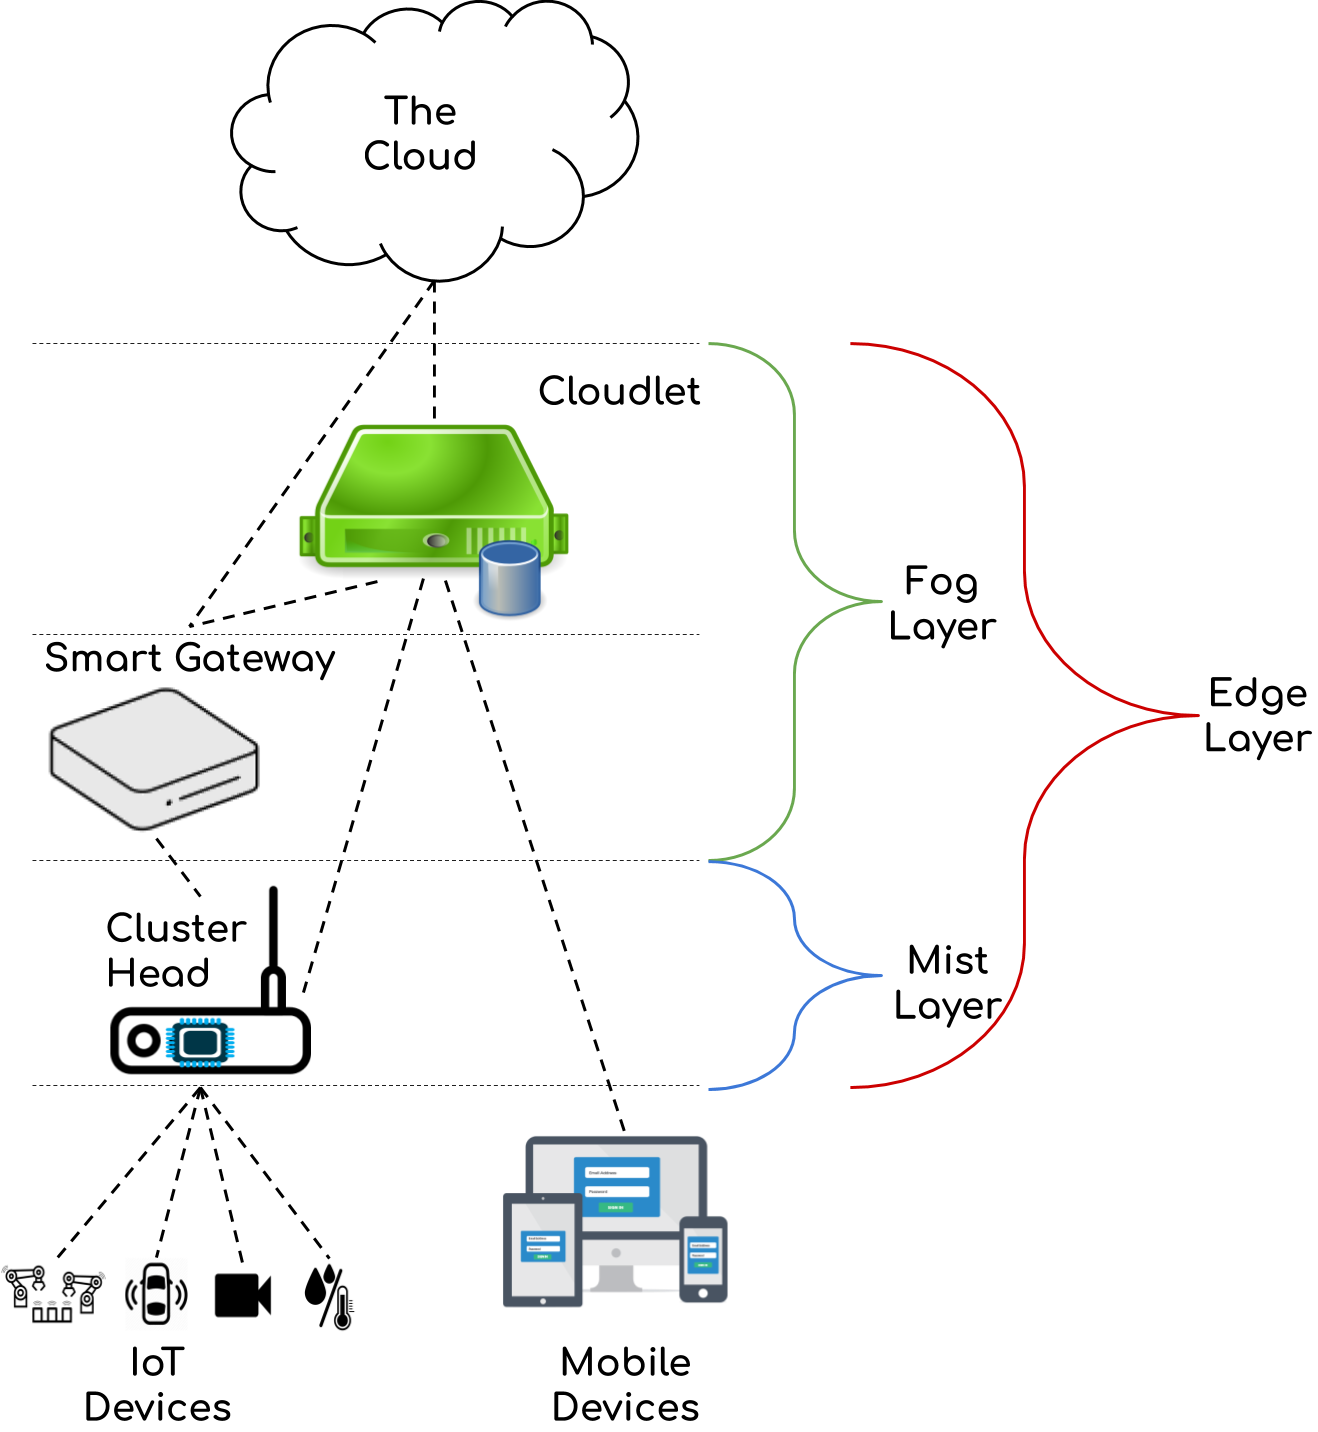
\includegraphics[scale=0.2]{figures/network-topology-3-layer.png}
    \caption{Three tier layer network topology, similar to \cite{nsa2017NextWaveIoTDef}}
    \label{fig:networkTopology3Layer}
\end{figure}

The cloud is well defined and understood. It describes the readily available computing resources over the Internet not managed by the user. The other layers and devices are not so well understood and defined separately.
\textbf{\textit{Constrained Device}}\\
Constraint devices are an elementary part of the IoT making up the "things"\cite{contstraintDevicesTerminology}.
They can have three main purposes. Either sensing or actuating (or both), where sensing is the 
passive action of measuring the environment (e.g. a motion detector) and actuating is the active action of influencing the environment (e.g. control of pressure in test tube). Or, finally, they can be smart objects enhancing the interaction between other smart objects and people.
They are usually defined by their limitation, mainly, small computing power (CPU, RAM, storage etc.) and limited power supply and operate in constrained network using protocols like BLE and ZigBee. \\[5mm]
\textbf{\textit{Smart/mobile devices}}\\
Smart devices are not clearly defined in the academic literature. I will use the definition given by \citeauthor{poslad2011smartDevices}\cite{poslad2011smartDevices}, to clearly divide them from constrained devices which this thesis will be concerned with. They are traditional computing devices and "tend to be multi purpose ICT devices"\cite{poslad2011smartDevices}, examples are mobile phones (smart phones) or tablets. They connect to the rest of the infrastructure directly but are free to move between networks. They also often rely on battery power and, importantly, are mainly end user devices. This has important privacy implication, a major factor for edge computing.\\[5mm]
\textbf{\textit{IoT Cluster Head}}\\
IoT Cluster Heads are defined by their very limited processing power. They are used to combine multiple sensors or actuators, but do not perform powerful operations. The line between IoT Cluster Heads and IoT Gateways is constantly moving as devices get more powerful and software more efficient. In this paper, IoT Cluster Heads are defined as devices which are used to read and control IoT devices but are not powerful enough to run containers or Kubernetes.
\textbf{\textit{IoT Gateway}}\\
IoT gateways are the connection between constrained devices and the cloud. I will use the term IoT gateway and not only gateway to stress its relation with IoT. They are usually connected to a network, either local or the the Internet. They facilitate inter-network and intra-network communications and because smart devices and especially constrained devices often communicate via wireless and non-Internet protocols, IoT gateways often translate protocols "between wireless sensor networks [...] and traditional communication networks"\cite{zhu2010iotGatewayDefinition}.
In recent years IoT Gateways have become a major field of interest and new research. As these devices got more powerful, developers started using them for pre-processing and data gathering locally at the edge.
IoT gateways can take a wide variety of forms. They can be simple L2/L3 routers or more powerful devices. Importantly, they are situated at the edge of a network.\\[5mm]
\textbf{\textit{Edge Layer}}\\
The edge layer is a term used to describe all resources sitting at the edge of the network. They do not interact with their environment directly only through IoT or mobile devices. This line started to fade, when mobile devices where used to control IoT devices directly. In this research I will stick to definition that edge layer devices are no user facing devices.\\[5mm]
\textbf{\textit{Fog Layer}}\\
The fog layer and consequently fog computing is a term used to describe the logical extension of traditionally cloud resources to the edge. These devices are still connected to the overall system and are an active part in the data processing pipeline. Fog computing enables repeatable structure on the edge for better and more scalable performance.
\textbf{\textit{Mist Layer}}\\
The mist layer is not logically connected to the cloud and both are not part of the same system and function independently of each other. It can be that the cloud can indirectly control the mist layer through the fog devices but importantly the mist layer does not do tasks which were traditional done in the cloud. \\[5mm]
\textbf{\textit{Edge cluster}}\\
Edge clusters are two or more edge devices working together where one device needs to be powerful enough to run a full control plane of the cluster technology. With emerging technologies like tiny builds of a full Kubernetes cluster, e.g. K3s from Rancher Labs\cite{k3sLight14:online}, this is becoming increasingly easier and more popular.
\footnote{Rancher provides a 40MB Kubernetes binary and claims that 500MB of RAM is sufficient 
it stable.}.\\
\textbf{\textit{Edge node}}\\
Edge nodes are defined as nodes "that act as an end user portal for communication with other
nodes in cluster computing"\cite{Whatised17:edgeNodeDef}. The other nodes can either be edge nodes as well or cloud nodes. Importantly, edge nodes do not need to be able to run their own control plane.
\subsection{Existing Solutions} \label{sec:existingSolutions}

Traditionally, edge devices were isolated cluster heads mainly forwarding traffic from their slaves to the cloud. Today, they are an integral part of the data flow pre-processing data and executing part of the business logic. But, there are still no coherent architectural as well as technological standards. In this section we will compare widely adopted and developed solutions in the industry to detect similarities and differences. The solutions also differ in age and 

% https://scholar.google.com/scholar?cluster=13680069378267225814&hl=de&as_sdt=0,5
% https://www.pac-online.com/sites/pac-online.com/files/upload_path/PDFs/Thema_des_Monats_Juni_2017_IoT_Plattformen.pdf
% https://blog.bosch-si.com/bosch-iot-suite/lessons-learned-using-kubernetes-in-iot-deployments/

\subsubsection{Bosch IoT Gateway Solutions}
\comment{https://www.bosch-iot-suite.com/service/gateway-software/}
The Bosch IoT Gateway Software\cite{BoschIoT13:online} is the "oldest" software analyzed. It is based on the OSGi technology\cite{osgiDefintion25:online}, which is an aliance driven project from the Open Services Gateway initiative (OSGi). It defines a set of specifications (with reference implemetation and tests) for a dynamic modular system based on so called bundles, third party software, running on the Java Virtual Machine (JVM)\footnote{This means it is possible to use other languages apart from Java which can run in a JVM, e.g. Kotlin.}. It is important to note that Bosch also supplies a cloud part which is based on Kubernetes.\\
The OSGi framework consists of a layered model shown in \cref{fig:osgiLayerModel}. 
\begin{figure}[h!]
    \centering
    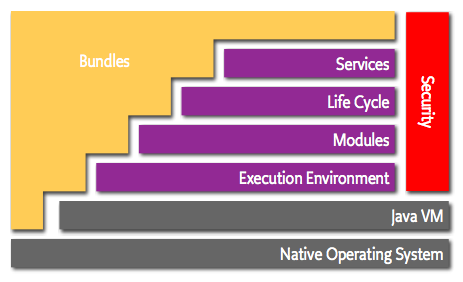
\includegraphics[scale=0.8]{figures/layering-osgi.png}
    \caption{From the official OSGI documentation\cite{osgiFrameworkArchitec22:online}.}
    \label{fig:osgiLayerModel}
\end{figure}
The Service layer interconnects the bundles making it possible for them to communicate via plain old java objects (POJO).The Life-Cycle layer handles the the state of the application (start, stop, update and uninstall). The Modules layer defines how an application can import and export code and the Execution Environemnt defines which methods and classes are available in a specific environemnt. Finally, the Security layer encompasses all other layers and handles for example code authentication, the digital signing of jar files, file access restrictions, certificates and more.\\
To the authors best knowledge there are currently five frameworks implementing the OSGi model besides the Bosch IoT Gateway Software\cite{BoschIoT13:online}. In a blog entry from 2015 Bosch compares the OSGi technology to other gateway solutions and says it "is the only one with clearly defined specs and an open specification process behind them"\cite{boschBlogOSGi69:online}. Boschs solution is proprietary and tailor made for edge-computing devices with IIoT in mind\cite{OSGiforIoTBlog27:online}. It runs on Linux, Windows, mac OS, Android, and VxWorks and according to Bosch more than 40 different gateway devices\cite{BoschIoT13:online}. The software is stable at major version 9 and still under heavy development. It is presented as exemplary software by the OSGi Alliance for IoT Gateways \cite{exampleIoTGateweOSGi:online} and thus used in this report. \Cref{fig:boschIoTGatewaySetup} shows where Boschs IoT solution is situated in the IoT environment. Bosch provides the OSGi framework implementation for the gateways and additional features for the cloud to ease the management of the gateways and store the accumulated data.
\begin{figure}[h!]
    \centering
    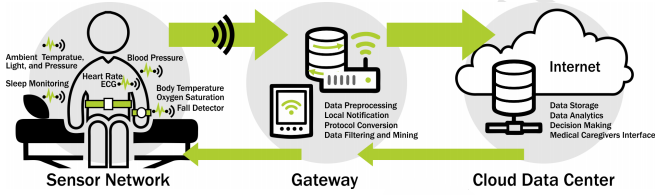
\includegraphics[scale=0.8]{figures/iotSetup.png}
    \caption{From the official Bosch documentation \cite{BoschIoT13:online}.}
    \label{fig:boschIoTGatewaySetup}
\end{figure}
Moreover, it supports a wide variety of communication protocls, BLE, ZigBee and MQTT, just to name a few. The main restriction is the JVM support for a protocol.  

\subsubsection{ioFog}
ioFog is one of the older projects in this report, with the first official release in 2016\cite{ioFogMainBlog:online}. Similarly to the OSGi framework it provides a runtime environment for applications, mainly intended for microservices. In addition, it includes a message bus, dynamic configuration of the microservices, and remote debugging\cite{ioFogMainBlog:online}. It runs on (almost) all Linux distributions and only requires Docker to be installed. In their official system requirements they only recommed using a Raspberry Pi as a worker node and not to run the Controller and Connector infrastructure \cite{ioFOgQuickStart:online}.
\Cref{fig:ioFogComponent} shows the fog computing layers in more detail.
\begin{figure}[h!]
    \centering
    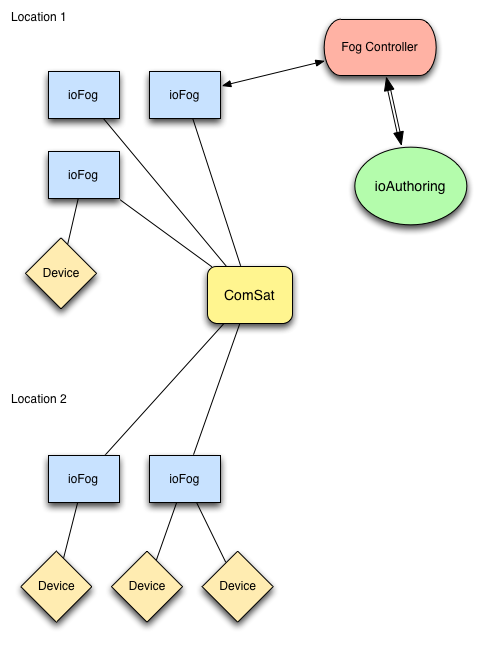
\includegraphics[scale=0.4]{figures/ioFog-Component_Diagram.png}
    \caption{hallo}
    \label{fig:ioFogComponent}
\end{figure}\\
The ioAuthoring application and the ioFog instances provide orchestration and management of the microservices. They are the main interaction points between the administrator and the system.
The fog computing software agent, called "ioFog", runs on various operating systems and provides a universal runtime for the IoT microservices. It includes a Software Development Kits (SDKs) in multiple programming languages to provide developers with the convenience of programming against standardized objects. The communication between different ioFog instances is facilitated through an internetworking utility that runs on popular Linux distributions, called "ComSat". Finally, for testing a tool for mimicking the fog computing runtime is included as well.\\
In a recent blog post from Mike Milinkovich, the Executive Director of the Eclipse Foundation Inc., he announced the initial availability of ioFog features that make any Kubernetes distribution edge-aware. He continuous saying that "these native Kubernetes enhancements are in the process of being contributed to the Eclipse ioFog open source project.", so not all features are available in the stable release as of the time of writing. But essentially, the ioFog Kubernetes APIs would provide standardized way of communication between the Kubernetes API Server and the ioFog instance.

\subsubsection{Docker Edge Solution}
Docker is commonly known for its containerization software and is often confused with the containers themselves (like google for search). The core container runtime, containerd, was donated by Docker to the Cloud Native Computing Foundry (CNCF) in 2017\cite{containerDonationDocker79:online} which manages and develops it now. Now, the company Docker focuses on providing an ecosystem around containers making them easy to deploy, secure and replicate. Recently, Docker announced a new partnerships with ARM and  a new strategy for edge devices.\\
\Cref{fig:dockerEdge} shows the Docker Edge Solution in context. 
\begin{figure}[h!]
    \centering
    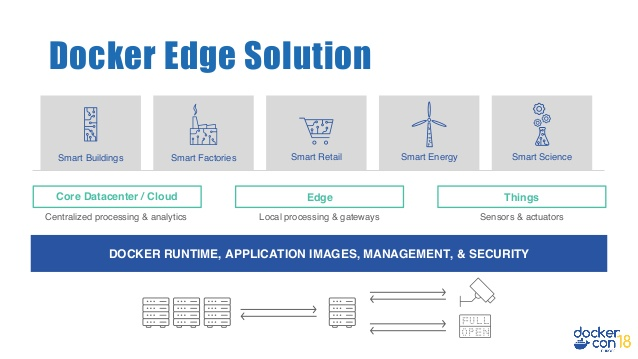
\includegraphics[scale=0.65]{figures/docker-edge-solution.jpg}
    \caption{Docker Edge solution .}
    \label{fig:dockerEdge}
\end{figure}
The solution consists of a few different products from its enterprise solution focusing on security, scalability/deployability and easy of use. The components are the same, but the edge focus is on fault tolerance and platform support, hence the new partnership with ARM. A core component of the suit is the docker registry, which can be mirrored/replicated on many difference servers for scaleability and fault tolerance. The edge registry can function without constant communication with the rest of the swarm. In case of no connection, the registry will only pull images which it already posses. As edge devices often have limitted disk space, docker only synchronizes promoted images on these nodes. Similarly to tags in git, promoted images are signed images that are explicitly marked as production ready. \cref{fig:dockerRegistryForIoT} shows registry management in the cloud (on the left) vs. on the edge (on the right).
\begin{figure}[h!]
    \centering
    \noindent\makebox[\textwidth]{
    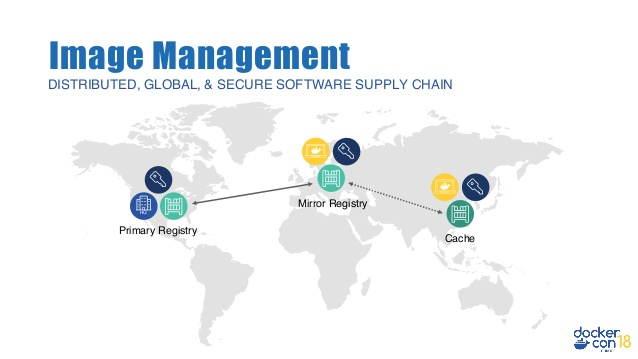
\includegraphics[width=(\textwidth+4cm)/2]{figures/docker-edge-computing-with-docker-enterprise.jpg}
    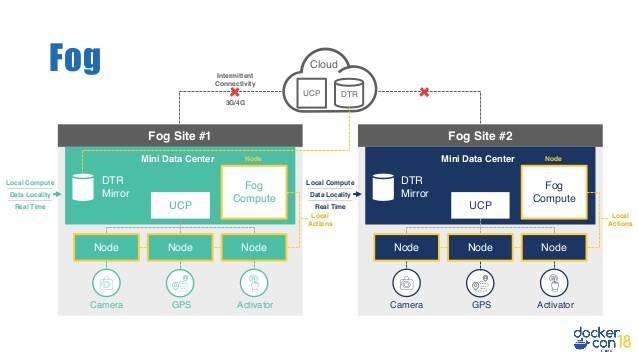
\includegraphics[width=(\textwidth+4cm)/2]{figures/docker-edge-registry-mirror.jpg}}
    \caption{The Docker registry in the cloud (left) vs. on the edge (right).}
    \label{fig:dockerRegistryForIoT}
\end{figure}
Whereas the cloud registry is build high availability (HA/LB) of the nodes in the swarm with fault tolerance against other nodes being unavailable, the edge registry is designed to have fault tolerance on it's own Internet access. In case of no connection it works as a standalone component, but synchronizes itself when it has a connection.\\
Importantly, the Docker Edge Solution is not a standalone solution, but integrates into the Docker ecosystem enabling remote management.

\subsubsection{K3s}
K3s is a "lightweight" kubernetes\footnote{Kubernetes is also known as k8s, hence the name k3s.} fork developed by Rancher\cite{rancherMainPage:online}. Similarly to Kubernetes and containerd, k3s is an open source project under the official management of the CNCF. It is also part of the Kubernetes IoT Edge working group explicitly aiming at bringing kubernetes related technologies to the edge. K3s is also a Certified Kubernetes distribution, meaning it confirms with the Kubernetes API standards. One of its big selling points is the good support for ARM64 and ARMv7 (targeting the Raspberry Pi and other smaller/less powerful single board computers). The traditional Kubernetes development is focused around the x86\_64 architecture, with limitted, and often untested, support for ARM, especially ARMv7. The co-founders of Rancher and developers behind k3s actually state in a webinar that half their development effort went into ensuring that all features they wanted work seamlessly on ARM\cite{k3sTalk:online}.\\
On their k3s product page \url{https://k3s.io/} Rancher describes the fork as follows:
\begin{displayquote}
Easy to install. A binary of less than 40 MB. Only 512 MB of RAM required to run.
\end{displayquote}
So k3s is not only significantly smaller than the full fledged Kubernetes install, but also requires significantly less resources at run time. It achieves this by mainly slimming down Kubernetes only including what they deem important for the edge. Because of the huge popularity of Kubernetes, it needs to support legacy code, drivers etc. K3s is free to break compatibility with older versions and the developers can instead focus on slimming down the code base much as possible. The lead developer, Darren Shepherd, said:
\begin{displayquote}
\textit{"We took Kubernetes and ripped out every single feature we didn't want.\cite{k3sTalk:online}"}
\\[1pt]
\raggedleft{{\rm --- Darren Shepherd}}
\end{displayquote}
K3s also integrates all process required by Kubernete, the Kubernetes master, Kubelet and containerd under one system process which requires less memory in total. \\
Another important aspect of k3s is its purpose to run on single as well as multi-node clusters. This is in stark contrast to Kubernetes, which is intended to run inside a cluster and it's fault tolerance model is build around on a multi-node cluster structure. Running a single node cluster is possible, but requires the tainting of the master node and is describe as "cheap and easy, but is not production grade" in the official documentation\cite{singleNodeKubernetesNotProductionDocumenhtation:online}.

\subsubsection{Kubeedge}
Kubeedge is another project inside the Kubernetes IoT Edge working group and thus build with Kubernetes in mind. It is a relatively young project to extend native containerized application orchestration and device management to the Edge. It is based on two parts, the cloud and the edge and (mainly) developed by Huawei, which at the time of writing could be reason for future complications because of recent US sanctions against the company.\\
The kubeedge system is shown in \cref{fig:kubeedgeStruct}.
\begin{figure}[h!]
    \centering
    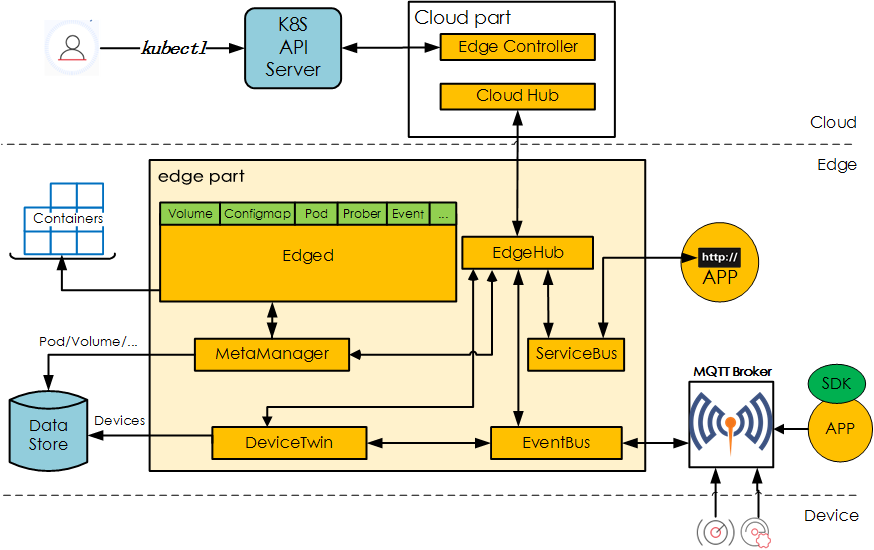
\includegraphics[width=(\textwidth+4cm)/2]{figures/kubeedge_arch.png}
    \caption{The Kubeedge system design.}
    \label{fig:kubeedgeStruct}
\end{figure}
The cloud part is built upon Kubernetes and provides support for application deployment, metadata synchronization and networking all through the Kubernetes API Server. The cloud and edge part communicate via web sockets. This means by design a good connection to the server is expected and the intend of the authors is to enable Fog computing. It is built upon Kubernetes and provides core infrastructure support for networking, application deployment and metadata synchronization between cloud and edge.\\
The edge part is not based on Kubernetes but uses similar concepts: Pods, volumes, events and more. It provides a life cycle management for containers and supports MQTT for communication for additional components. It also stores and synchronizes the device status to the cloud and has a query interface for local applications.

\subsubsection{Conclusion}
Only recently have industry behemoths like, Docker, Huawei, Bosch, Siemens, Red Hat, VMware and more\cite{K8sattheEdgeContectOnWorkingGroup:online} started to develop and, more importantly, concentrate their efforts on integrated IoT Gateway solutions. This lack of standardization is also acknowledged by the developers themselves ``While the problems at the IoT edge — connectivity, manageability, scalability, reliability, security — are being solved as point solutions by enterprises and ecosystem players, there is a need for a foundational industry-wide standard for managing distributed IoT workloads.''\cite{ioFogK8sBlog:online}\\
\Cref{tab:shortSotaSoftware} shows how the different solutions analyzed in this section compare to each other in key aspects.
% \footnote{An extended version can be found in the appendix.}
\begin{table}[h!]
% \hspace*{-2cm}
    \begin{center}
        
    \noindent\makebox[\textwidth]{
\resizebox{\columnwidth}{!}{%
\begin{tabular}{l|lll p{2.5cm} lllll}
                  & \begin{tabular}[c]{@{}l@{}}Open\\Source\end{tabular} & \begin{tabular}[c]{@{}l@{}}Centralized \\ control plane\end{tabular} & SW   &  Protocols  & \begin{tabular}[c]{@{}l@{}}System Req\\ control plane\end{tabular} & \begin{tabular}[c]{@{}l@{}}System Req\\ worker node\end{tabular} & \begin{tabular}[c]{@{}l@{}}Container\\based\end{tabular} & \begin{tabular}[c]{@{}l@{}}Kubernetes\\ in cloud\end{tabular} & \begin{tabular}[c]{@{}l@{}}Kubernetes\\ on edge\end{tabular} \\ \cline{1-10} 
Bosch IoT         & No                                                                                                                             & Yes (cloud)                                                                                                                                  & Java & ZigBee, Z-Wave, BLE and more        & Server grade                                                                                                                               & Edge grade                                                                                                                               & No                                                                                                                                & Some                                                                                                                                  & No                                                                                                                                   \\
ioFog             & Yes                                                                                                                            & Yes (cloud)                                                                                                                                  & Java & ZigBee, Z-Wave, BLE and more        & Server grade                                                                                                                               & Edge grade                                                                                                                               & Yes                                                                                                                               & Some                                                                                                                                  & No                                                                                                                                   \\
Docker\\Enterprise & No                                                                                                                             & Yes (cloud)                                                                                                                                  & Go   & ZigBee, Z-Wave, BLE and more        & Server grade                                                                                                                               & Edge grade                                                                                                                               & Yes                                                                                                                               & No                                                                                                                                    & No                                                                                                                                   \\
K3s               & Yes                                                                                                                            & Yes (both)                                                                                                                                   & Go   & Only IP based protocols             & Edge grade                                                                                                                                 & Edge grade                                                                                                                               & Yes                                                                                                                               & Yes                                                                                                                                   & Yes                                                                                                                                  \\
Kubeedge          & Yes                                                                                                                            & Yes (cloud)                                                                                                                                  & Go   & MQTT and IP. More planned & Server grade                                                                                                                               & Edge grade                                                                                                                               & Yes                                                                                                                               & Yes                                                                                                                                   & No                                                                                                                         
\end{tabular}}}
    \caption{Summary of the analyzed software.}
    \label{tab:shortSotaSoftware}
    \end{center}
\end{table}
It is important to bear in mind, that the Bosch IoT solution as well as ioFog are significantly older than the other projects. Boschs IoT solution is based on the OSGi framework. It provides isolation evolving around the JVM. This enables it to be platform independent, that is as long as the OS provides a JVM. ioFog which is almost three years old as of time of writing (June 2019) and already relays on containers, specifically a Docker runtime, for its deployment.\\
As the second last column shows all solutions, except for Docker Edge, use Kubernetes as their orchestration platform and control plane of choice. ioFog and Bosch IoT Edge are currently updating their solution while Kubeedge and K3s where designed from the ground up with Kubernetes in mind. However, only K3s tries to bring Kubernetes to the edge as well. This also means, that all solutions require different hardware requirements for the control plane, usually server grade hardware running containers, and more resource efficient solutions for the edge. \\
It is also important to note that all newer solutions, Docker Edge Solution\footnote{As the source code is not publicly available, this is speculative based on the fact that the main programming language for Docker is Go.} K3s and Kubeedge are developed in the Go programming language. Older systems are mainly based on Java as it enables code to run on every JVM supported platform. It is also important to note, that containers give developers freedom of programming language. The Bosch IoT Edge Solution and its use of the OSGi framework force developers into using a JVM compatible programming language. Docker points out that its solution runs on MacOS and Windows, however, both rely on Linux system calls.\footnote{Docker on Windows uses the WSL 2.0 in the future which translates Linux system calls to Windows system calls and increases performance a lot compared to emulated solutions as done on MacOS.}.\\
Another important aspect is protocol support. Here, the OSGi framework is clearly ahead as it has complete access to the system hardware, due to the JVM and also 



% From a design perspective, this is very similar to containers, where isolation is provided by Cspaces and Namespaces instead of process ID. Containers need access to communication 

% Giving access to devices like  Blt sigbee is a security issue.



\comment{
Should I include Azure IoT Edge as managed cloud iot gateway offering????\\

The problems at the IoT edge, connectivity, manageability, scalability, reliability, security, are being solved as point solutions by enterprises and ecosystem players, there is a need for a foundational industry-wide standard for managing distributed IoT workloads.


What is the purpose of this section?\\
problem area: what is actually the problem with the current system? hint into solution\\
competitor anaylsis: compare different approaches to solve the management and security of IoT gateways as well as solutions inside the individual categories. 


}
\section{Analysis} \label{sec:analysis}
The analysis section will be split into different segments: Container technology, Kubernetes, the IoT/edge stack, and, finally, the requirements for the implementation. Essentially, the analysis will be the foundation of the implementation giving reason to the major design choices described in the requirements. The critical areas for the edge are: memory and disk space constrains, security, speed, protocols, loadbalancing and internet access.\\
In this thesis I will deploy containers to the edge using Kubernetes to determine what is still missing and what features already enable Kubernetes to make this possible. Standardization of the edge is going to be key.

\subsection{Containers}
Containers first surfaced in 2007 with the release of Linux Containers (LXC). They provide an abstraction and isolation layer to the software they are supposed to run. Basically, a container is packaged software that runs independent from the underlying system. They are created at runtime from container images, which are packaged, standalone executable software including everything the main application needs to run (code, runtime, system tools, libraries and settings)\cite{containerDefinition:online}. Since 2007, there has been considered development of containers, especially by Docker, a company developing the same named application which is often used synonymously for containers. Docker than donated its main container runtime environment, called containerd, to the open source community and later, in late 2017, announced the first major release of containerd. https://blog.docker.com/2017/12/cncf-containerd-1-0-ga-announcement/ This was significant news, as the docker software was already widely used and it marked the start of an independent open source standard for containers. \\
Today, containers are the building blogs of the cloud and power almost all distributed applications. Craig McLuckie, the lead product manager cloud computing product at Google, said in a panel discussion during the Linux collaboration summit in Febraury 2015:
\begin{displayquote}
\textit{\textbf{\large{``}}}
\textit{This containers revolution is changing the basic act of software consumption. It’s redefining this much more lightweight, portable unit, or atom, that is much easier to manage... It’s a gateway to dynamic management and dynamic systems.}
\textit{\textbf{\large{''}}}
\end{displayquote}
It is important to note, that while the cloud saw the first transformation from containers the edge is part of the same dynamic system and also needs dynamic management.\\ 
The rest of the section will discuss the advantages of using containers focusing on the edge component. I will show the advantages and disadvantages of containers in terms of memory management, portability and security, and ways to combat the disadvantages. To keep the thesis concise I will not explain how containers in greater detail\footnote{For more information on this topic see Docker's website  \url{https://www.docker.com/resources/what-container} and containerd \url{https://containerd.io/}} .

\subsubsection{Resource consumption}
Memory consumption from containers is always greater than bare metal deployments. By design containers share little with the default namespace, apart from system resources, like the kernel. It is possible to give containers access to host directories, but this often breaks their design philosophy of being stateless and portable. The solution is to include the libraries, tools, certificates necessary to run the application in the container itself. It is not hard to image with multiple containers memory and RAM consumption can easily exceed the system resources of edge devices, e.g. the Raspberry Pi’s. For example, deploying the latest official openJDK container consumes 470MB. Source and byte code and dependencies add on top of this. Compiled language are at a huge advantage in this regard. Go is one such example and used in this thesis. It can be cross-compiled to machine code for most CPU architecture compatible with Linux and results in one application file without any dependencies. Multi-stage builds allow to have one container to build the application and only copy relevant files into the final image. This eliminates any unused files and is often used in combination with the \textit{scratch} image. This is the base image for all other containers and is basically an empty file structure consuming no memory. According to Docker it ``is most useful in the context of building [...] super minimal images''\cite{scratchImageDockerD65:online}.\\
Combining these these techniques can result in far lower memory and RAM consumption, but also better security (discussed in the next section). In the implementation, \cref{sec:testService} \nameref{sec:testService}
hard topic, as this is not needed in the cloud
\subsubsection{Security}
Security is one of the biggest challenges in IoT. In 2016 a botnet with over 600k infected devices, primarily edge and IoT devices, overwhelmed several high-profile targets like the DNS provider Dyn with massive distributed denial-of-service (DDoS) attacks. This caused a temporary outage of their DNS servers rendering many webpages, among others  Twitter, Spotify and Amazon, temporally inaccessible. To combat malicious attacks certain methods have been developed. I will only analyze the direct container security aspects as they are always applicable for containers. Other methods, like specifically developed OSs and securing the CI/CD pipeline are not discussed at this point.\\
Most registries allow for overriding of images. In the implementation \cref{sec:testService} \nameref{sec:testService} I will use the \textit{hello} service for testing. It's current version, v5arm, is saved on the Docker image hub and can be pulled with the link \textit{jonas27/hello:v5arm}. However, each image also has an image digest, a cryptographic signature ensuring that the image in question is the actual image. In production (not done in this thesis) an image should always be pulled based on the image digest, also called "Pinning-by-Digest". In the case of the test service the link would then be \textit{jonas27/hello:sha256:725355347bc2eae8f7c9ab9dd09b9ef2c884b3458c693978f5408785aef1fb72}. This simple technique not only improves security but also guarantees that each container is derived from the same image, but it also guarantees that every instance of the service is running exactly the same code and combats race conditions.\\
In a recent talk at the "Container Security Conference" Andy Martin, co-founder of control plane, noted ``The root of all evil is unnecessarily running processes or containers as root''\cite{RootlessContainerSecurityTalk0:online}. By default, all images use the root user as default user. However, the root user can read, write and run all files in all directories. In the beginning of 2018 a new vulnerability on Kubernetes was discovered giving containers with volume mounts the ability to access data outside the volumes sub-path. The root user would thus have unlimited access to the host resources. To combat this, the user can be changed to a newly created user. 

Scratch user
binary no reverse engineering
no modification possible.



\comment{
https://www.iotforall.com/containers-on-the-edge/

 They isolate the application runtime and the 

Containers and Cloud: From LXC to Docker to Kubernetes

}

\subsection{Kubernetes}
Kubernetes is the de-facto standard for container orchestration and the main aspect of this thesis. In this section I look at the fundamentals of Kubernetes and highlight the best strategies to run it on edge devices. I will also look what is currently missing to make it a truly edge ready. With that being said, Kubernetes has so many features and tools that discussing them all is impossible. The same is true for its ecosystem which is constantly evolving and adding even more layers to the mix. I will try to keep this section short and concise, but it will come at the cost of complexity.\\
IIoT has accelerated the need for fog computing and the industry is set to develop a container based orchestration tool, tightly integrated with Kubernetes. The Kubernetes IoT edge working group was set up specifically to find the optimal Kubernetes strategy for the edge. However, it is not clear, whether the solution will be Kubernetes itslef or a more specialized tool. In this thesis I will argue that Kubernetes is the way forward as it already posses many of the features that are need for the edge.\\ 
I will start with addressing the elephant in the room, single-cluster vs multi-cluster. I will then analyze the core components of Kubernetes, mainly the kubelet, together with other resource configurations. Afterwards, I will focus on the optimal deployment strategy, how to control resources on the edge and node selection. Finally, I will look at the security aspect of Kubernetes and conclude with recommendations for the implementation.

\subsubsection{Single Vs Multi-Cluster}
Google recently revealed a new and much hyped product, Anthos\cite{TechnicalAnthosGoogle66:online}. Its a combination of many services, but most importantly it lets people easily manage hybrid clouds. Google describes it as follow: "Anthos is a modern application management platform that provides a consistent development and operations experience for cloud and on-prem environments"\cite{TechnicalAnthosGoogle66:online}. Google provides an installer for on-prem but onece installed Google itself manages the cluster including updates and troubleshooting. Not only is it a multi-cluster solution, but it also integrates the clusters with Istio service mesh and other neat features. Open source Kubernetes only has the multi-cluster management solution called Kubernetes Cluster Federation.



\subsection{The IoT/Edge Problems}
Resource consumption and orchestration are big problems in the cloud and equally so for the edge. Containers and Kubernetes can be adopted to consume less resources and Kubernetes enables remote orchestration of on-prem nodes. But, because of the heterogeneity of the edge, it faces even more problems. Discussed in this section will be load balancing, protocol conversion and traffic shaping.\\ Not thoroughly discussed in this section will be the issue of ultra low latency. In an updated performance assessments of containers the authors found that containers introduce almost no overhead over a native deployment\cite{felter2015updatedPerformanceContainers}. Hence, gateways running Linux can in most cases use containers without a problem. 

\subsubsection{Load Balancing}
Load balancing in a distributed environment is difficult as the ingress node needs a complete network topology at any given moment in time. This is one of the reasons why Kubernetes refreshes its node status so often. If a external request comes in at the master it needs to know where to forward the traffic. In the previous section \cref{sec:singleVsMultiCluster} \nameref{sec:singleVsMultiCluster} I discussed the advantages and disadvantages of multi-cluster in contrast to single clusters and load balancing is a perfect example why the decision has to be carefully weight. A full Kubernetes cluster on the edge comes with the advantage of having a full control plane on the edge and, thus, being able to do load balacing on the edge, with for example Istio Ingress Gateay. If the master nodes taint were to be removed it could even become part of the operational unit of the cluster.\\
But having a cluster at edge comes with its downside. It needs a lot more management than a single cluster setup. It consumes drastically more resources than having only worker nodes and it needs a stable connection between the cluster nodes to work. But if resource consumption on the master is not an issue Kubernetes coupled with a load balancer provide more features and safeguarding than most other load balancers do. Kubernetes always ensures that pods inside the cluster are healthy and reachable and if a pod goes down, Kubernetes will automatically spawn a new one. The internal load balancer can use this information and always route to an available pod. Other gateways like, Kong API Gateway, can not do this. Also with Istio it becomes possible to do very fine grained traffic routing, somthing I will discuss in the next section \cref{} \nameref{}.\\
Finally, internal load balancing\footnote{Load balancing withing one node.} is possible through normal API gateways and the deployment of multiple pods listening on different ports. For example, one NGINX container could function as load balancer for 5 docker containers in the background. In Kubernetes this could be solved with affinities. As soon as a node runs certain pods, a load balancer could be automotically side loaded.
\subsubsection{Traffic Control and Shaping}
Traffic control and traffic shaping are very interesting edge topics. In Kubernetes each pod can be assigned incoming and outgoing bandwidth rates. But other tools extend this functionality and open up new possibilities. Istio, a service mesh mainly developed for Kubernetes, injects a sidecar proxy to fine tune the traffic of each container. It makes it possible to do rate limiting, control headers, reroute connection, change retries attempts, circuit breaking, mirroring and more while not changing the application code. Additionally, it is also able to encrypt traffic inside the mesh without the application knowing about it and gather all the telemetry data of the cluster. \\
With Kubernetes and tools extending its capabilities it is possible to do both traffic control and traffic shaping on a fine grained level. But, especially Istio, comes at the cost of additional overhead and the operator has to decide if the added functionality are worth the performance hit. Without Istio traffic control and shaping is only possible through the Kubernetes Ingress and thus in multi-cluster solutions.\\
Finally, Kubernetes is only meant to work with the Internet protocol stack and is only meant to operate within the clusters boundaries. So the actual communication with the IoT devices can not be controlled or shaped with Kubernetes. 
\subsubsection{IoT Protocols and Protocol Conversation}
Kubernetes was designed for the Inernet and not for the heterogenity of the edge. This means the IoT gateway must either implement a DHCP server, the IoT device must have a static IP or the communication is facilitate outside Kubernetes realm and then converted by a service to IP. Please note that lower level protocols for establishing a connection between two devices, e.g. Ethernet, Wi-Fi (IEEE-802.11) or Bluetooth, are not discussed at this point. The most common IoT protocols are MQTT, CoAP, AMQP and DDS. In contrast to Internet protocol stack, these technologies do not need to support legacy systems and can thus concentrate on whats important in IoT, very low energy, distribution and memory consumption. I will mainly compare MQTT\cite{MQTT50:online} to CoAP\cite{CoAP—Con75:online} because of the their vast usage and academic literature. \Cref{fig:mqttVsCoap} shows side by side the architecture of MQTT and CoAP. Both are based on machine to machine (m2m) communication and are optimized for the IoT space, but the similarities stop there.
\begin{figure}[h!]
    \centering
    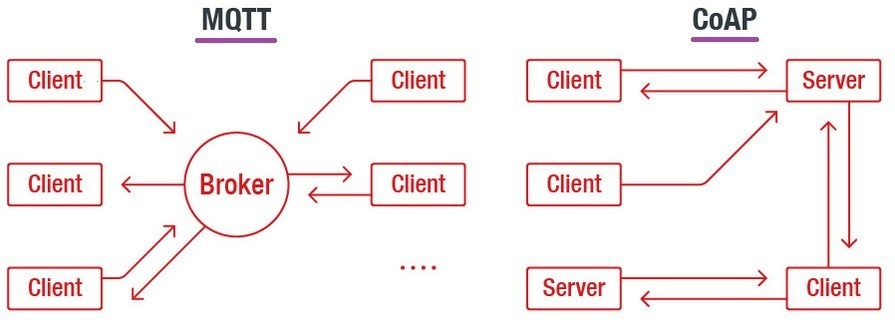
\includegraphics[scale=0.45]{figures/mqtt-vs-coap.jpg}
    \caption{MQTT and CoAP architecture side by side\cite{COAPvsMQTT27:online}.}
    \label{fig:mqttVsCoap}
\end{figure}
MQTT is based on the publish-subscribe massaging pattern which relies on a central entity, called broker, to enable communication between multiple nodes, mainly IoT devices. CoAP on the other side is a classic client server protocol and is based on the Internet stack. Researches compared the two standards and found "MQTT messages experienced lower delays than CoAP for lower packet loss and higher delays than CoAP for higher packet loss"\cite{MQTTvsCoAPAnalysisIEEE}. They also found that the message overhead for small messages is significantly lower at 25\% or less for CoAP compared to MQTT for reliable message transmission. Whereas in MQTT the broker needs additional services to convert the data to Internet compatible standards, CoAP is already able to communicate directly through the Internet. This opens up new possibilities including decentralized communication in subnets.\\
Finally, the data serialization can be even more important than the protocol itself. With the advent of RESTful services JSON soared in popularity. It is human readable but not very space efficient. When researches compared JSON to protobufs they found huge message size differences between the two, shown in \cref{fig:jsonVsProtobufs}.
\begin{figure}[h!]
    \centering
    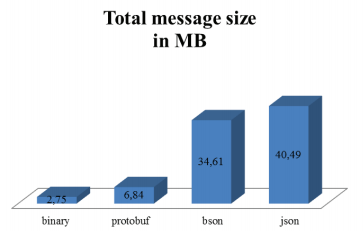
\includegraphics[scale=0.45]{figures/jsonVsProtobufs.png}
    \caption{Memory consumption of different serialization methods\cite{}.}
    \label{fig:jsonVsProtobufs}
\end{figure}
The researches conclude "the Protocol Buffers are a serious candidate for standardized way of communication in field of Internet of Things"\cite{jsonVsProtobufs}.

\comment{
protocol conversation
Traffic shaping
Load balacing
}



\subsection{Requirements Specification}
The requirements are based on insights from existing solutions and the use cases and provide a guideline for the implementation in the next section. I will only create functional requirements as non-functional requirements "indirectly related to the overall success of the system"\cite{aauFunctionalRequirements} and are usually confirmed by intense testing. As this thesis aim is to provide an exploratory example of using Kubernetes at the edge specific constraints are not important. 

The functional requirements are listed and ordered via the MoSCoW method in \cref{tab:functionalRequirements}. The main purpose in this thesis is to have a working prototype showcasing Kubernetes on the edge. The MUST requirements are the once deemed necessary to fulfill this and have a "M" (for MUST) in the "Class" field of the table. The SHOULD requirements are abbreviated by "S" are features which do not make or brake the system, but for an industry wide standard they should be present. This mainly includes security and networking aspects. The COULD requirements are mainly features which add extra business functionality and make the system easier to use. The WOULD requirements are features which are either not directly related to the product or out of scope.
% Please add the following required packages to your document preamble:
% \usepackage[normalem]{ulem}
% \useunder{\uline}{\ul}{}
% \begin{table}[]
\clearpage
\setlength\LTleft{-2.5cm}
\begin{longtable}{l p{3.5cm} p{0.8cm} p{12.5cm} }
\multicolumn{4}{l}{Functional Requirements}       
                                                                                                                                                                                                                              \\
ID                      & Name                                    & Class  & Description                                                                                                                                                                                                                         \\ \hline




101                     & Isolated applications                   & M      & Each application has to function on its own. It has to handle database errors and communication errors in a non fatal way.                                                                                                          \\
102                     & Isolation to host computer              & M      & The application has to be as isolated from the host environment as possible.                                                                                                                                                        \\
103                     & Minimal dependencies                    & M      & The application has to have minimal runtime dependencies. If the application is built on the edge device the compile time dependencies have to be minimal as well.                                                                  \\
104                     & Cross compilation                       & M      & The edge applications has to be able to be cross-compiled.                                                                                                                                                                          \\
105                     & Small images                            & M      & The footprint of the application has to be small as possible                                                                                                                                                                        \\
106                     & Use different users                     & M      & Each application should be run by different users. If one userspace is compromised it does not effect the other applications.                                                                                                       \\
107                     & Use non root user                       & M      & The application should not run with root priviledges except when really needed.                                                                                                                                                     \\
108                     & Isolate the application context         & M      & The application process has to be isolated. Only if the application must access host resources should they be available to the application.                                                                                         \\
109                     & Secured application code                & M      & The application source code has to be secure in case of a databreach on the node. A malicious attacker should not be able to reconstruct the source code even when he gets access to it.                                            \\
110                     & Trusted applications                    & W      & The edge application would be verified before the deployment.                                                                                                                                                                       \\
111                     & Centralized orchestration               & M      & The operator should only need to tell a central configuration tool in the cloud how the system should looks like. The cloud has to then orchestrate the edge automatically.                                                         \\
112                     & Automatic application deployment        & M      & Based on a new configuration the edge device has to be able to automatically get a copy of the new application shut down the old application and deploy the new one.                                                                \\
113                     & Isolate edge from cloud                 & C      & The cloud and the edge could work independently so without a data connection. This is in case the edge is powerful enough to run its own control plane and the setup is big enough to justify the overhead of running multicluster. \\
114                     & Isolated cloud environments             & S      & Developers should only have access to the resources they need.                                                                                                                                                                      \\
115                     & Resource quotas                         & M      & The operators must be able to set resource quotas on applications and groups of applications.                                                                                                                                       \\
116                     & ARM compatible edge                     & M      & The orchestration tool on the edge has to be able to run on (slower) ARM powered devices.                                                                                                                                           \\
117                     & Node fault tolerance                    & M      & The state of each node must be synchronized in the system so that in case of an error the last operable state can be recovered.                                                                                                     \\
118                     & Decentralized edge storage              & W      & When possible each edge device would synchronization important data with other edge devices in a distributed database.                                                                                                              \\
119                     & Traffic prioritization                  & S      & System critical information should be prioritized in case of congestion.                                                                                                                                                            \\
120                     & Whitelist connections                   & S      & Only cluster internal communication should be allowed to access applications on the pods.                                                                                                                                           \\
121                     & Application independent traffic shaping & S      & The traffic for each application should be contralable without changing the application code.                                                                                                                                       \\
122                     & Secure traffic within cluster           & S      & The communication between the nodes inside the cluster should be secure. This includes the edge to cloud communication.                                                                                                             \\
123                     & Internet compatible IoT protocol        & M      & The IoT protocol must to be compatible with the Internet protocol. This enables addressing of IoT devices through the Internet in case of a static IP.                                                                              \\
124                     & Secure traffic with IoT devices         & S      & The communication between the IoT gateway/edge device and the IoT device needs to be secure.                                                                                                                                        \\
125                     & Efficient message compression           & M      & The messages between the edge device and the IoT device must be efficiently compressed to save resource and enhance speed.                                                                                                          \\
126                     & Energy efficient transmission           & M      & The transmission between the edge and the IoT device must be energy efficient.                                                                                                                                                      \\
127                     & Automatic updates                       & S & The edge device should be able to update the IoT device. The update process is intiated in the cloud but the operator does not have to do local configurations. The system updates alone once initiated.                            \\
128                     & OTA updates                             & C      & The IoT device updates could support OTA updates.                                                                                                                                                                                   \\
129                     & Verified updates                        & W  & The IoT device updates would be verified before installing them.                                                                                                                                                                   




\end{longtable}
\label{tab:functionalRequirements}
% \end{table}
\clearpage

\comment{
First list and then clissify (MoSCoW

An example of a functional requirement would be:
A system must send an email whenever a certain condition is met (e.g. an order is placed, a customer signs up, etc).

Docker:
From Scratch
no privileges, only if really important and only what is needed
no root, only if necessary
Compiled language
Only necessary files in container

Kubernetes:
Single cluster as small
Docker Hub mirror
Use a edge ready kubelet
Use namespace to separate into virtual clusters

IoTEdgeProblems
Assign priorities for traffic
Use Istio to secure communication and for traffic shaping
Use CoAP to explore kubernetes possiblities.
Use protobufs.






}





\comment{In fact, a new Kubernetes IoT Working Group is investigating how it can provide a consistent deployment model for IoT cloud and IoT Edge.
https://blog.bosch-si.com/bosch-iot-suite/why-the-iot-needs-kubernetes/

WHTA is important for edge? 
small containers
internet access (function without)
security
Speed (kubelet)
protocols


}
\clearpage
\section{Implementation} \label{sec:implementation}
The implementation is based on one Kubernetes master in the cloud and and one worker on-premises, at the edge. The master runs on a virtual private server (VPS) from Contabo\cite{online:ContaboWebsite}. 
It has four cores, a minimum of 10 gigabyte of RAM, more then the official Kubernetes requirments\cite{kubernetesRequirementsInstall:online}, and runs Ubuntu 18.10. The worker is a raspberry pi (RPi) model 3b+ on bare metal as here performance is critical. It has one gigabyte of RAM and runs on ARMv7, a 32-bit architecture. It meets the Kubernetes system requirements for workers on paper, but it is generally not recommended by the Kubernetes developers to run Kubernetes for production purposes on the device. The RPi is one of the most popular single-board computers and often used in IoT project, I use it in this thesis as well.

I will divide the implementation in different stages for better understanding. In stage one I setup the system, installing the edge device and joining it to the master. In stage two, I will deploy an example application to the edge device controlled from the Kubernetes master. I will explain in more detail the build steps for the containers and how it is deployed. In stage three the IoT setup will be deployed. This includes a CoAP server on the edge and microcontroller sending data to that server. 


\subsection{Kubernetes Installation}
The Kubernetes master installation is well documented and did not pose any troubles. For completion of this thesis I will briefly mention the additional components installed on the master. Kubernetes has no default networking implementation, thus I installed Flannel\cite{coreosFlannel:online}, one of the simplest and most widely used networking fabrics specifically designed for Kubernetes. It runs a small binary called \textit{flanneld} on each node and provides networking between nodes and pods\footnote{The specifics of Flannels networking are outside this thesis scope, for more information see \url{https://blog.laputa.io/kubernetes-flannel-networking-6a1cb1f8ec7c}}. For administrative purposes I also installed the Kubernetes Dashboard.

The Raspberry Pi Foundation recently released an update to Raspbian (the RPi OS) called buster, which does dropped support of the aufs-dkms kernel modules, which are dependencies of kubeadm and containerd. The online community advised in forums to avoid the dependency but if possible switch back to the older version of Raspbian called stretch. Out of time concerns, I switched back to the old version. 

I switched the official Kubernetes kubelet with the kubelet binary from Ranchers K3s called Hyperkube. \Cref{fig:kubeBinaries} shows the size of the binary files of three most important components of Kubernetes, kubeadm, kubelet and kubectl.
\begin{figure}[h!]
    \centering
    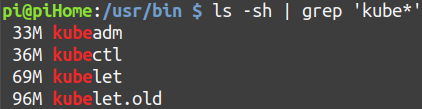
\includegraphics[scale=0.5]{figures/kubeBinariesSize.png}
    \vspace*{-0.3cm}
    \mycaption[The Sizes of the Kubernetes Binaries.]{\\ Note, \textit{kubelet} is the K3s hyperkube binary and \textit{kubelet.old} is the official kubelet bianry.}
    \label{fig:kubeBinaries}
\end{figure}
In total the official binaries are 165 megabyte large and the kubelet (\textit{kubelet.old} file) takes almost half the space. Using the K3s build of kubelet (\textit{kubelet} file) brings the total amount to 138 megabyte saving almost 20\% of space in addition to its other benefits discussed in \cref{sec:Kubernetes} \nameref{sec:Kubernetes}. The full installation procedure can be found in the repository of this thesis for replication and validation.

Finally, the effects on the system resources are two folds, the native applications and the running containers. The Raspberry Pi has 926MB total memory and a 1.4 GHz quad-core CPU. Firstly, \cref{fig:kubernetesResourceConsumption} shows the resource usage of the native applications
\begin{figure}[h!]
    \centering
    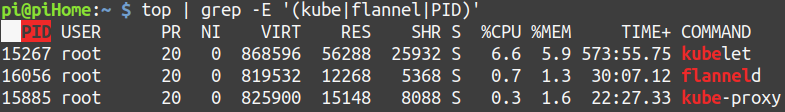
\includegraphics[scale=0.5]{figures/kubernetesResourceConsumption.png}
    \vspace*{-0.3cm}
    \caption[The Resource Usage of native Kubernetes Components.]{Using the K3s hyperkube binary.}
    \label{fig:kubernetesResourceConsumption}
\end{figure}
The kubelet process uses 6.6\% of the CPU and 5.9\% of the memory. While the memory usage is consistent, the CPU usage varies a lot and can reach peaks of 16\%. Using the command
\begin{displayquote}
\textit{top | egrep --line-buffered '(kubelet|PID)' > /home/pi/kubeletHyper.txt }
\end{displayquote}
the cpu usage was tracked over 38 minutes with an average of 3.16 data points per second and a total of 7235 data points\footnote{The entire statistics can be found in the project files together with the source code.}. The average CPU usage in the time period was 10.3\%, the memory usage was constant.

Flanneld and kube-proxy both use less than 1\% CPU and 1.3\% and 1.6\% of memory, respectively. It is important to note that the container runtime is not included in that statistics. The resource usage of the Kubernetes relevant containers is shown in \cref{fig:kubernetesResourceConsumptionCut}\footnote{The figure is cut to fit the page. The full figure can be seen the appendix.}.
\begin{figure}[h!]
    \centering
    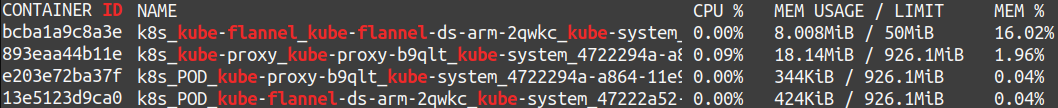
\includegraphics[scale=1.6]{figures/kubeContainerResourceUsageCut.png}
    \vspace*{-0.3cm}
    \caption[The Resource Usage of Kubernetes Containers.]{\\The command used is: \textit{docker stats | grep -E '(ID|kube|flannel)'}.}
    \label{fig:kubernetesResourceConsumptionCut}
\end{figure}
Flannel and kube-proxy consume 0.86\% and 1.96\% of the memory, respectively\footnote{flannel's limit is 50MB, hence the 16.02\% in the figure.}. The CPU usage of all containers is negligible at below 1\%. Adding up the numbers, after the installation Kubernetes uses 11.4\% of the CPU and 11.7\% of the total memory. This translates to 0.46GHz CPU usage, see \cref{eq:cpuTotal}, and 108.35MB memory usage, see \cref{eq:ramTotal}.
\begin{equation} \label{eq:cpuTotal}
    1.4GHz * 4 \; \textrm{(cores)} * 0.114 = 0.638GHz  \quad \textrm{(CPU usage)}
  \end{equation}
  \begin{equation} \label{eq:ramTotal}
    926.1MB * 0.117 = 108.354MB  \quad \textrm{(RAM usage)}
  \end{equation}
The memory consumption is especially concerning as swap needs to be disabled for Kubernetes to install. Swap is a partion in Linux used for paging. If disabled, memory can not be written to disk anymore which can lead to a memory overflow.
\subsection{Implementing a test Service} \label{sec:testService}
To test the Kubernetes setup I developed a simple go microservice called \textit{hello}. It listens on port 3000 and has three endpoints \textit{/hello/}, \textit{/hello/info} and \textit{/hello/path}. They don't implement any deeper logic but pose as an exemplary implementation for future services. I show exemplary Kubernetes configuration files and use this section to explain their meaning in more detail. For easier testability with cURL this microservice is based on json and not on protobufs.\\
\Cref{lst:dockerfileHello} shows the Dockerfile for building the microservice.
\lstset{
numbers=left, 
basicstyle=\footnotesize,
frame = single, 
language=Pascal, 
framexleftmargin=16pt,
% captionpos=b,
xleftmargin=2.3cm,
}
\begin{lstlisting}[linewidth=13cm, caption={Dockerfile for the Hello Application},label={lst:dockerfileHello}]
FROM golang:alpine as builder
EXPOSE 3000
COPY src .
RUN adduser -D -H -u 10001 scratchuser && \
    cd /go/main && \
    CGO_ENABLED=0 GOOS=linux GOARCH=arm GOARM=7 
    go build -a -installsuffix cgo -ldflags 
    '-extldflags "-static"' -o main .

FROM scratch
COPY --from=builder /etc/ssl/certs/ /etc/ssl/certs
COPY --from=builder /go/main/main /
COPY --from=builder /etc/passwd /etc/passwd
USER scratchuser
CMD ["./main"]
\end{lstlisting}
The code is cross-compiled in a builder container, which provides an isolated and replaceable build environment, this happens in line 1--8. Line 1 takes a fresh go alpine container with the latest go version. I then expose the port 3000 for the application to interact with its environment and copy the source code in the new container, line 2 and 3, respectively. Each new command produces a new temporary cached container, thus I the lines, 4--8, are all one \textit{RUN} command. It first adds a new user called \textit{scratchuser} without root privileges and the goes into the go main file directory and cross-compiles the application for ARMv7 (the last step is line 6--8). In lines 10--15, the final image is build. Line 10 initializes a new scratch container. This image is empty and thus uses a less memory and system resources. In lines 11--13 the relevant documents are copied in the new container. This includes the certificates from certificate authorities\footnote{They are important for encrypted connections.} (11), the application binary (12) and the user password (13). Line 14 switches to the scratchuser. This user has no root privileges and thus can never gain system control. Lastly, I specify the command run when a container based on the build image is run (15).\\
To see how important it is to use a scratch image as a base for memory purposes, consider \cref{fig:imageSizeComparison}. It shows just how much can be saved using this technique.
\begin{figure}[h!]
    \centering
    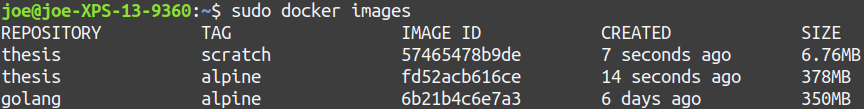
\includegraphics[scale=0.4]{figures/imageSizeComparison.png}
    \caption{The image sizes of the application.}
    \label{fig:imageSizeComparison}
\end{figure}
The go alpine image at the bottom is 350MB, the final image is a hefty 28MB bigger at 378MB (lines 1--8 in \cref{lst:dockerfileHello}). Copying the binary, the user files and the  certificates into a scratch image takes up only 6.76MB in total (lines 11--13). That is significantly smaller and with less overhead. When the container runs, only the binary is loaded and nothing else is running in the background. Contrast that to the alpine image where every time it is run, it starts a shell command line and includes an entire go build environment. The image is then tagged with a repository and tag name and pushed to the corresponding repository.\\
On the Kubernetes master I defined a service for the \textit{hello} application with the manifest shown in \cref{lst:serviceManifest}. It is an abstraction defining the guidelines how to access the pods inside a service, as the pods themselves are volatile\footnote{Each pod has a unique IP but Kubernetes does not guarantee for Pods and can reschedule pods at any moment}. It thus enables decoupling of the networking and the actual application from an outsiders perspective.
\lstset{
numbers=left, 
basicstyle=\footnotesize,
frame = single, 
language=Pascal, 
framexleftmargin=16pt,
% captionpos=b,
xleftmargin=2.3cm,
}
\begin{lstlisting}[linewidth=13cm, caption={The manifest of the \textit{hello} service.},label={lst:serviceManifest}]
apiVersion: v1
kind: Service
metadata:
  name: hello-service
  namespace: hello-namespace
spec:
  type: NodePort
  selector:
    app: hello
  ports:
    - name: http
      nodePort: 30001
      port: 3000
      targetPort: 3000
\end{lstlisting}
Line 5 tells the master that the service should be deployed in the namespace \textit{hello-namespace}. Line 6 specifies that each pod of this service should be accessible on the node it is scheduled on without going through the Kubernetes ingress resource. This is called nodeport and specified in line 12 to be \textit{30001}. Line 7 tells Kubernetes that the application corresponding to the service is called \textit{hello}. Finally, line 13 and 14 specify the ports the actual container expose.\\
For the actual state description of the application I use a \textit{Deployment} shown in \cref{lst:deploymentManifest}. A deployment specifies the desired state and the Deployment controller changes the actual state inside the cluster towards the desired state. 

\lstset{
numbers=left, 
basicstyle=\footnotesize,
frame = single, 
language=Pascal, 
framexleftmargin=16pt,
escapeinside=||,
xleftmargin=2.3cm,
}
\begin{lstlisting}[linewidth=13cm, caption={The Deployment Manifest of the \textit{hello} Application.},label={lst:deploymentManifest}]
apiVersion: apps/v1
kind: Deployment
metadata:
  name: hello-deployment
  namespace: hello-namespace |\Suppressnumber|
... |\Reactivatenumber{16}|
    spec:
      affinity:
          nodeAffinity:
            requiredDuringSchedulingIgnoredDuringExecution:
              nodeSelectorTerms:
                - matchExpressions:
                    - key: kubernetes.io/hostname
                      operator: In
                      values:
                        - pihome
        podAffinity:
          requiredDuringSchedulingIgnoredDuringExecution:
            - labelSelector:
                matchExpressions:
                  - key: env
                    operator: In
                    values:
                      - test
              topologyKey: "kubernetes.io/hostname"
      nodeSelector:
        pi: "hello" 
      containers:
        - name: hello
          image: jonas27/hello:v5arm |\Suppressnumber|
...
\end{lstlisting}

\comment{
Put this in Appendix

apiVersion: apps/v1
kind: Deployment
metadata:
  name: hello-deployment
  namespace: hello-namespace
spec:
  selector:
    matchLabels:
      app: hello
  replicas: 1
  template:
    metadata:
      labels:
        app: hello
        version: v5arm
    spec:
      affinity:
          nodeAffinity:
            requiredDuringSchedulingIgnoredDuringExecution:
              nodeSelectorTerms:
                - matchExpressions:
                    - key: kubernetes.io/hostname
                      operator: In
                      values:
                        - pihome
        podAffinity:
          requiredDuringSchedulingIgnoredDuringExecution:
            - labelSelector:
                matchExpressions:
                  - key: env
                    operator: In
                    values:
                      - test
              topologyKey: "kubernetes.io/hostname"
      nodeSelector:
        pi: "hello"
      containers:
        - name: hello
          image: jonas27/hello:v5arm
          imagePullPolicy: Always
          ports:
            - containerPort: 3000

}



Line 3 and 4 specify the name and namespace of the deployment. Lines 17--34 specify the pod affinities, which places a constrained on where a certain pod can be scheduled. Similarly, anti-affinities constrain a pod to where can not be scheduled\footnote{I deployed another pod to the node beforehand with the correct label}. Lines 18--25 specify a node affinity "it allows you to constrain which nodes your pod is eligible to be scheduled on, based on labels on the node"\cite{affinitiesKubernetes:online}.
Lines 26--34 specify the pod affinity. Pods of the deployment will only be scheduled on nodes containing a pod with the specified label. This enables orchestration based on other pods. Lines 35 and 36 specify the single node a deployment should be scheduled on. These three methods can be used together but have to chosen carefully. Finally, line 37--39 specify the container which should be deployed inside a pod (the port selection is hidden).\\
With this configuration it is possible to clearly specify the nodes a deployment should be scheduled on. I omitted how to accomplish it via namespace, which has many benefits to it as well. However, deployments, the resource type used in this section, are volatile deployments and should thus only be used for stateless application, like the \textit{hello} application. Stateful pods require the resource type \textit{StatefulSet} and pods supposed to run on every node require the resource type \textit{ReplicaSet}, see \cref{sec:statefulvsdeploymentvsBLAAAA} for more information.

\subsection{System Implementation}
The implemented system is kept simple by using only one device at each network layer to reduce the overall system complexity. The architecture is shown in \cref{fig:actualSetup}. The IoT device, a esp32, is connected to a button and a light, the RPi makes up the edge layer and the VPS the cloud layer.
\begin{figure}
    \centering
    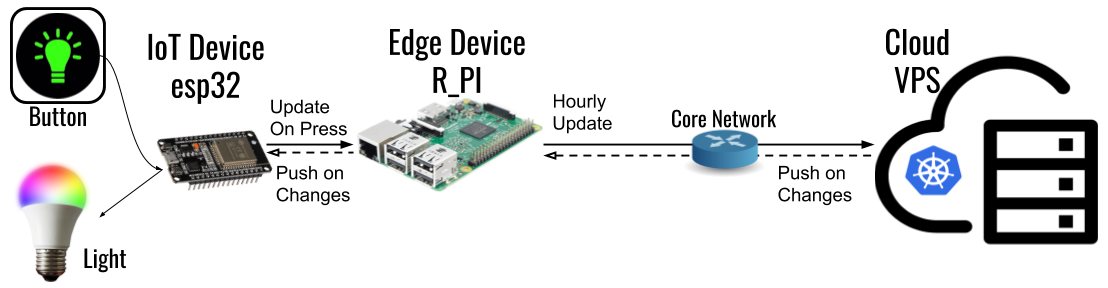
\includegraphics[width=\textwidth]{figures/actualSetup.png}
    \caption{The implemented system.}
    \label{fig:actualSetup}
\end{figure}
On the edge, all devices are directly connected either through wire or WiFi and are only dependent on each other to provide the normal functions. The expected round trip time (RTT) for a given signal should be rather low translating into an immediate response. In more extensive examples, the RPI could first check if pressing the button is even permissible and only then turn on the light/machine etc. In \cref{fig:actualSetup} the solid arrows stand for communication instantiated by the system and the dashed arrows communication instantiated by external changes. The systems internal communication always goes up, from the IoT devices to the cloud, whereas system external communication goes the other way around. It is also expected that the system internal communication happens far more frequently than the system external one.

\Cref{fig:actualImplementationSetup} uses the same layout as \cref{fig:implementationSetup} but shows the actual system implementation. Comparing it to the desired system under \cref{sec:desiredSystem} shows that major and minor changes following the classification of the requirements had to made as technology and time did not allow for a full implementation.

\begin{figure}[h]
    \centering
    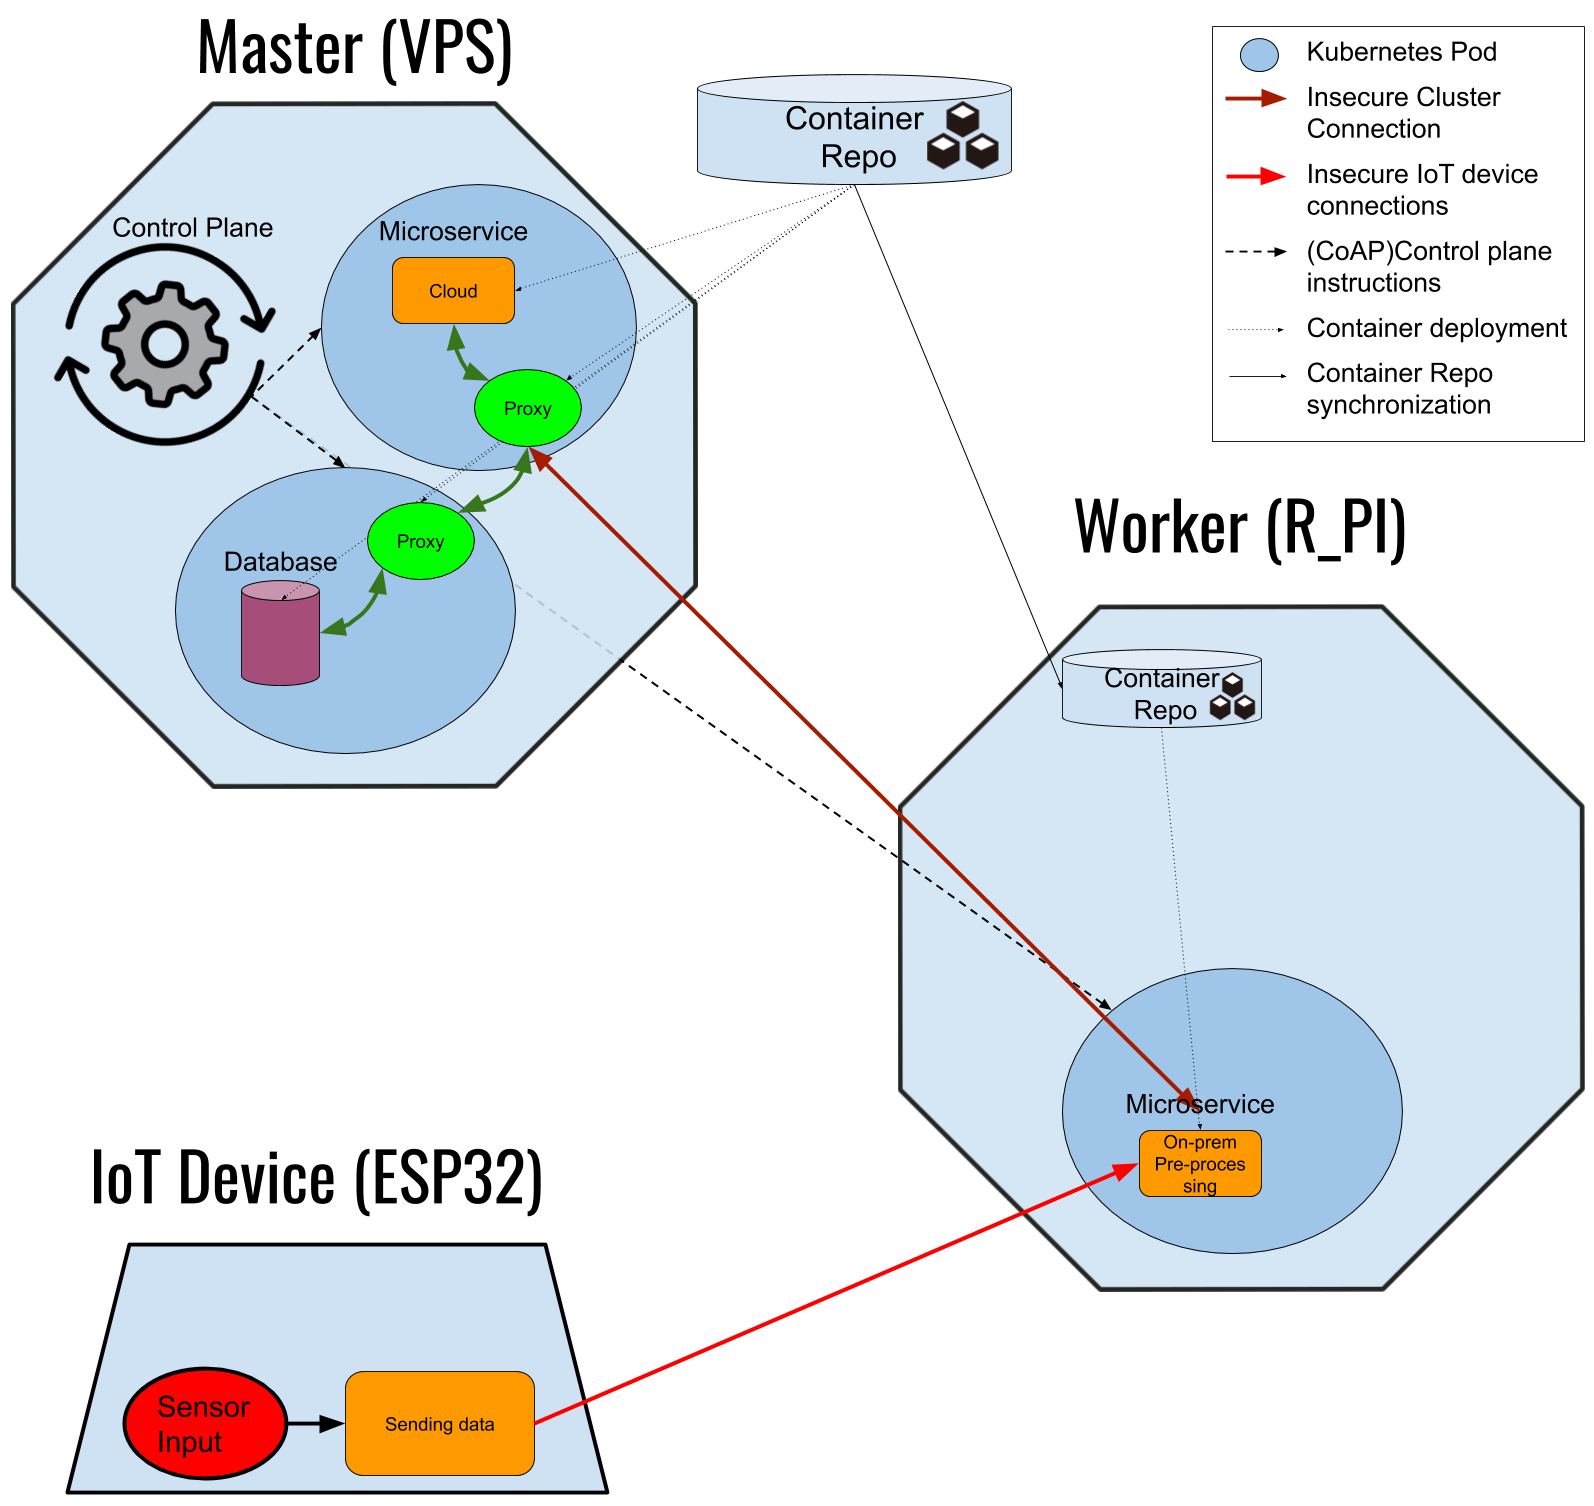
\includegraphics[width=\textwidth]{figures/actualImplementationSetup.png}
    \caption{The actual system architecture of the implementation.}
    \label{fig:actualImplementationSetup}
\end{figure}

The cloud part is unchanged from the desired setup. The edge part had to be adopted due to technical issues. The Istio envoy proxy does not compile for the ARM architecture yet. Istio provides traffic shaping and routing, default mutual TLS encryption between services, an extensive ingress gateway and more. Kubernetes is already capable of some of these things but Istio is a far more potent tool. It makes it impossible to reroute network traffic from the application to another destination and importantly the traffic between the edge and the cloud will not be encrypted. The envoy team is working on a patch for ARM devices but until then another solution has to be found. Using human produced certificates is not a good idea, especially for small project as the certificates have to be kept up to date, should be rotated and mutual TLS is hard to implement.

Similarly, the CoAP librarby for esp32 does not support DTLS yet. The developers are aware of it and are working on fixing it. Protobufs are base 128 encode message which provides a shielding against to most rudimentary attacks, but it is not a security mechanism to rely on. Finally, due to time issues and prioritization the update service for the IoT device was not been completed.

Apart from the automatic updates for the edge device, the networking and encryption issues, all requirements labeled as SHOULD or MUST have been successfully implemented. This means by pressing a button a user can turn on or off a light. In the background, this data is send from the esp32 to the RPI, which processes the data and sends a usage statistic of the light in defined time intervals to the server for further processing and storage. The system can also change the state of the light automatically from a centralized input field. Further, the administrator can update the specifications for all cluster internal resources (edge or cloud) and the system works towards implementing this specifications. It also means, in case of failure, e.g. an application crash on the edge, the system can reschedule this application. 

\begin{figure}[h]
    \centering
    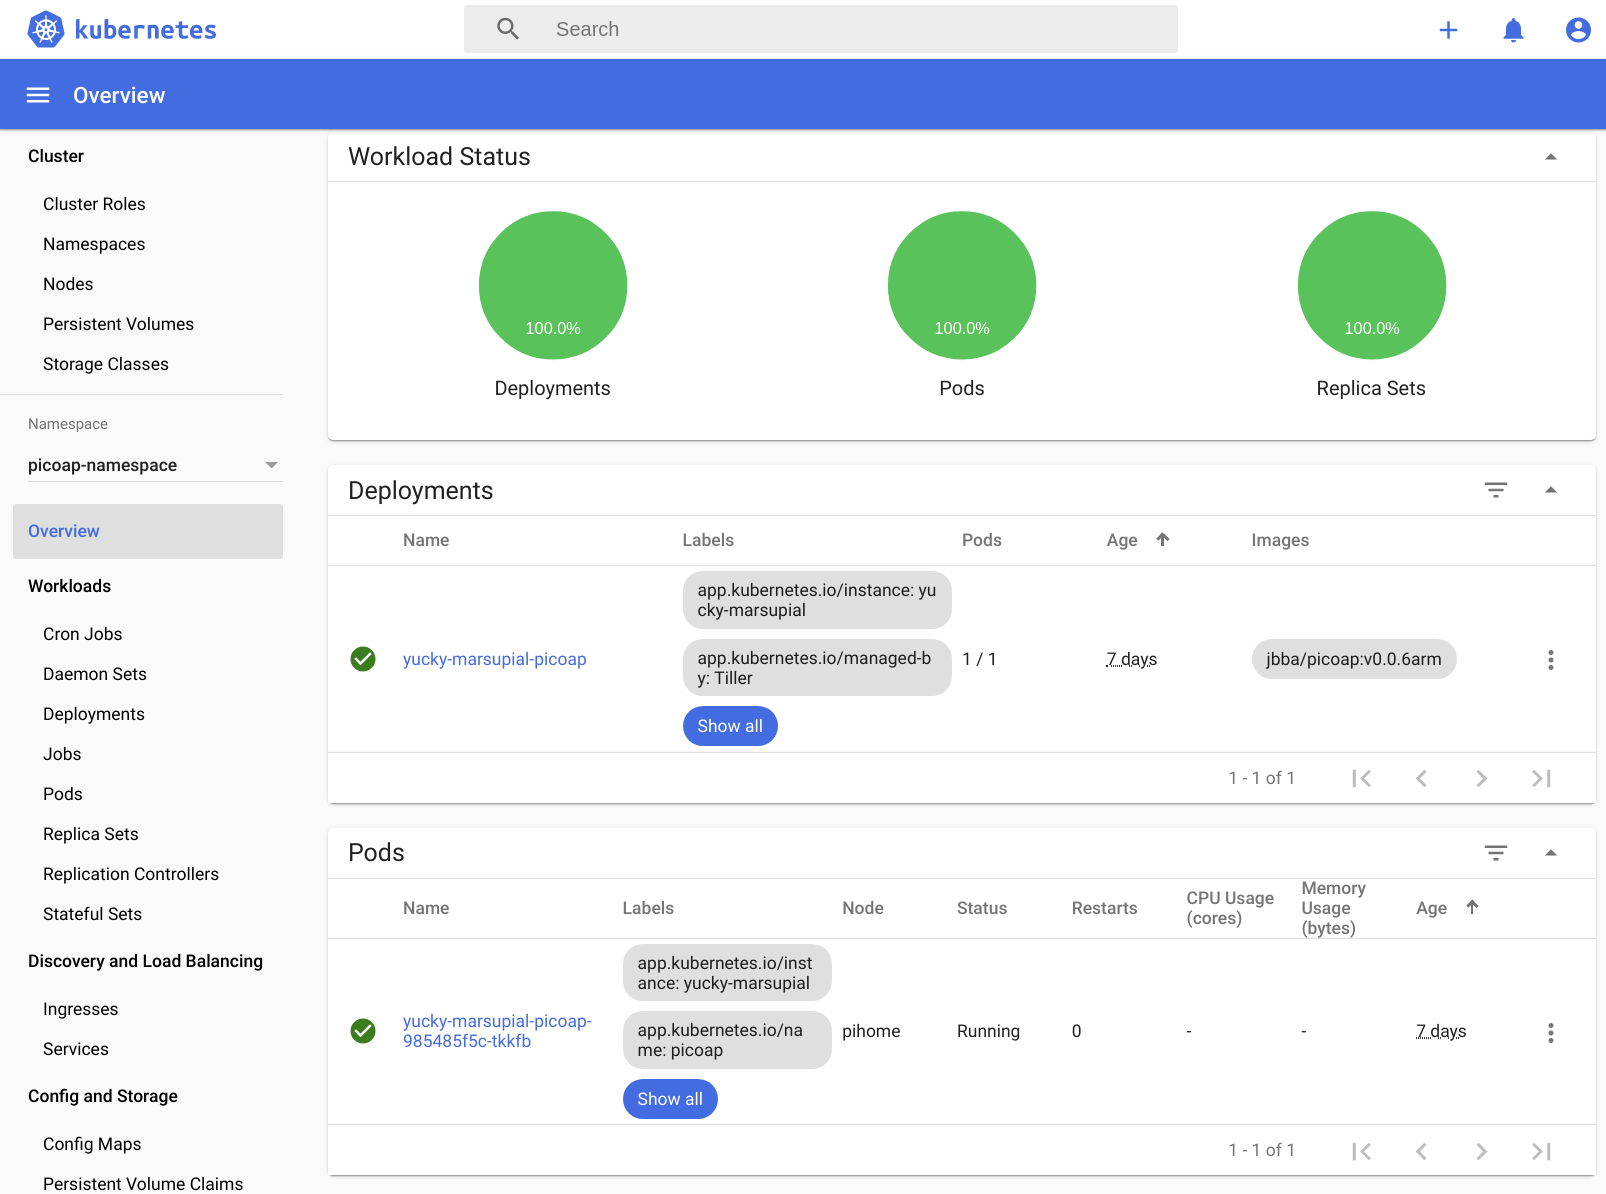
\includegraphics[width=\textwidth]{figures/dashboardK8s.png}
    \caption{The Kubernetes Dashboard showing the Edge Application.}
    \label{fig:dashboarK8s}
\end{figure}

\Cref{fig:dashboarK8s} shows the Kubernetes dashboard of the running application. It shows that the deployments, pods and replica sets are all working as they should. More services for the same namespace would show up here as well. To see the status of the resources in other namespaces it is enough to change to that namespace, provided the permissions are granted. This is the beauty of Kubernetes, it not only helps deploying applications but also provides extensive data about their status and always tries to restore a working state.



\comment{
\bgroup\obeylines
Kubernetes in the cloud
Node running locally with HiveMQ on a raspberry pi
HiveMQ is running as container
Static vs non static ip (only static ip atm)
connected to esp32 devices
\egroup
}





\comment{
Kubeedge
OTA update to esp32
https://randomnerdtutorials.com/esp32-over-the-air-ota-programming/




}
\clearpage

% \printbibliography[heading=bibintoc]
\clearpage

\let\svaddcontentsline\addcontentsline
\renewcommand\addcontentsline[3]{%
  \ifthenelse{\equal{#1}{lof}}{}%
  {\ifthenelse{\equal{#1}{lot}}{}{\svaddcontentsline{#1}{#2}{#3}}}}
 
 \pagenumbering{arabic}
 
% % \begin{appendices}
% \section{Structural factors}
% \begin{figure}[ht]
%     \centering
   
%     \label{fig:cat_strcut_mintzberg}
%     \caption{Elements of the Five Structural Configuration by Mintzberg}
%      \includegraphics[scale=0.4]{pictures/mintzberg_table.png}\\
%      Source: \cite{mintzberg1980structure}
% \end{figure}

% \clearpage
% \section{Morphological Box for Agillics version-control system}
% \begin{figure}
%     \centering
%     \caption{Morphological box for enterprise software 5.0}
%     \includegraphics[scale=0.4]{pictures/kees.png}\\
%     Source: \cite{kees2015characteristics}
%     \label{fig:kees}
% \end{figure}


% \end{appendices}


\end{document}